\documentclass[11pt,a4paper,oneside]{article}

% --- Core Packages ---
\usepackage[a4paper,margin=1.1in,footskip=0.5in]{geometry}
\usepackage[utf8]{inputenc}
\usepackage[T1]{fontenc}
\usepackage{amsmath,amssymb,amsfonts}
\usepackage[demo]{graphicx}
\usepackage{mathptmx}
\usepackage{courier}
\usepackage{booktabs}
\usepackage{xcolor}
\usepackage{listings}
\usepackage{tikz}
\usepackage{microtype}
\usetikzlibrary{shapes,arrows,positioning,calc,fit,shadows,backgrounds}
\usepackage[colorlinks=true, allcolors=blue!40!black, pdfborder={0 0 0}]{hyperref}

% --- Custom Colors ---
\definecolor{unizblue}{HTML}{003366}
\definecolor{unizlight}{HTML}{F1F5F9}
\definecolor{accent}{HTML}{334155}
\definecolor{divider}{HTML}{CBD5E1}

% --- Typography & Section Styling ---
\makeatletter
\renewcommand{\section}{\@startsection{section}{1}{\z@}%
    {-5ex \@plus -1ex \@minus -.2ex}%
    {3ex \@plus.2ex}%
    {\normalfont\huge\bfseries\color{unizblue}}}

\renewcommand{\subsection}{\@startsection{subsection}{2}{\z@}%
    {-4ex\@plus -1ex \@minus -.2ex}%
    {2ex \@plus .2ex}%
    {\normalfont\Large\bfseries\color{accent}}}

\newcommand{\makeuniztitle}{
  \begin{titlepage}
    \begin{tikzpicture}[remember picture,overlay]
      \node[anchor=north east, xshift=-1in, yshift=-1in] at (current page.north east) {
        \begin{tikzpicture}[scale=0.8]
          \draw[unizblue, line width=1.5pt] (0,0) -- (1,0) -- (1,1) -- (0,1) -- cycle;
          \draw[unizblue, line width=1.5pt] (0.2,0.2) rectangle (0.8,0.8);
          \fill[unizblue] (0.4,0.4) rectangle (0.6,0.6);
        \end{tikzpicture}
      };
    \end{tikzpicture}
    
    \begin{flushleft}
      \vspace*{5cm}
      {\fontsize{52}{62}\selectfont\bfseries\color{unizblue} UniZ\par}
      \vspace{0.8cm}
      {\huge\bfseries\color{accent} Systems Architecture \& Reference Manual\par}
      \vspace{1.2cm}
      {\color{divider}\rule{\linewidth}{1.5pt}}\par
      \vspace{1.2cm}
      {\large\sffamily\color{gray} Professional University Administration Ecosystem\par}
      
      \vfill
      
      {\small\sffamily\color{accent}
        \textbf{CONTRIBUTORS}\\\vspace{0.4cm}
        \begin{tabular}{@{}ll}
          \textbf{SreeCharan Desu} & --- \textit{infra and devops} \\
          \textbf{BhanuPrakash} & --- \textit{developer} \\
          \textbf{Seetharam} & --- \textit{cyber security} \\
          \textbf{Anand} & --- \textit{ai} \\
        \end{tabular}
      }
      \vspace{2cm}
      {\small\sffamily\color{gray} UPDATED: \today\par}
    \end{flushleft}
  \end{titlepage}
}
\makeatother

% --- Code Listing Style ---
\definecolor{codebg}{HTML}{F8FAFC}
\definecolor{codecomment}{HTML}{64748B}
\definecolor{codekw}{HTML}{0F172A}
\definecolor{codestr}{HTML}{334155}

\lstdefinestyle{unizstyle}{
    backgroundcolor=\color{codebg},   
    commentstyle=\color{codecomment}\itshape,
    keywordstyle=\color{unizblue}\bfseries,
    stringstyle=\color{codestr},
    basicstyle=\ttfamily\scriptsize,
    breaklines=true,                 
    numbers=left,                    
    numberstyle=\tiny\color{divider},
    numbersep=10pt,                  
    tabsize=2,
    frame=leftline,
    framerule=2pt,
    rulecolor=\color{unizblue!20},
    xleftmargin=20pt,
    showstringspaces=false
}
\lstset{style=unizstyle}

% --- Custom Info/Note Boxes ---
\usepackage[many]{tcolorbox}
\newtcolorbox{unizbox}[2]{
  colback=#1,
  colframe=gray!10,
  arc=0pt,
  boxrule=0.5pt,
  leftrule=3pt,
  title=\textbf{#2},
  coltitle=black,
  fonttitle=\small\sffamily,
  fontupper=\small,
  left=12pt,
  right=12pt,
  top=10pt,
  bottom=10pt
}

\begin{document}
\makeuniztitle

\begin{abstract}
\noindent This document provides the authoritative technical reference for the UniZ platform. UniZ is a high-performance, security-hardened university administration system designed for RGUKT. It leverages a modern microservices architecture, automated DevOps pipelines, and intelligent data processing to streamline campus operations. This manual combines high-level architectural oversight with direct implementation references.
\end{abstract}

\tableofcontents
\pagebreak

\section{System Overview \& Architecture}

\subsection{Microservices Mesh Topology}
\begin{figure}[h]
\centering
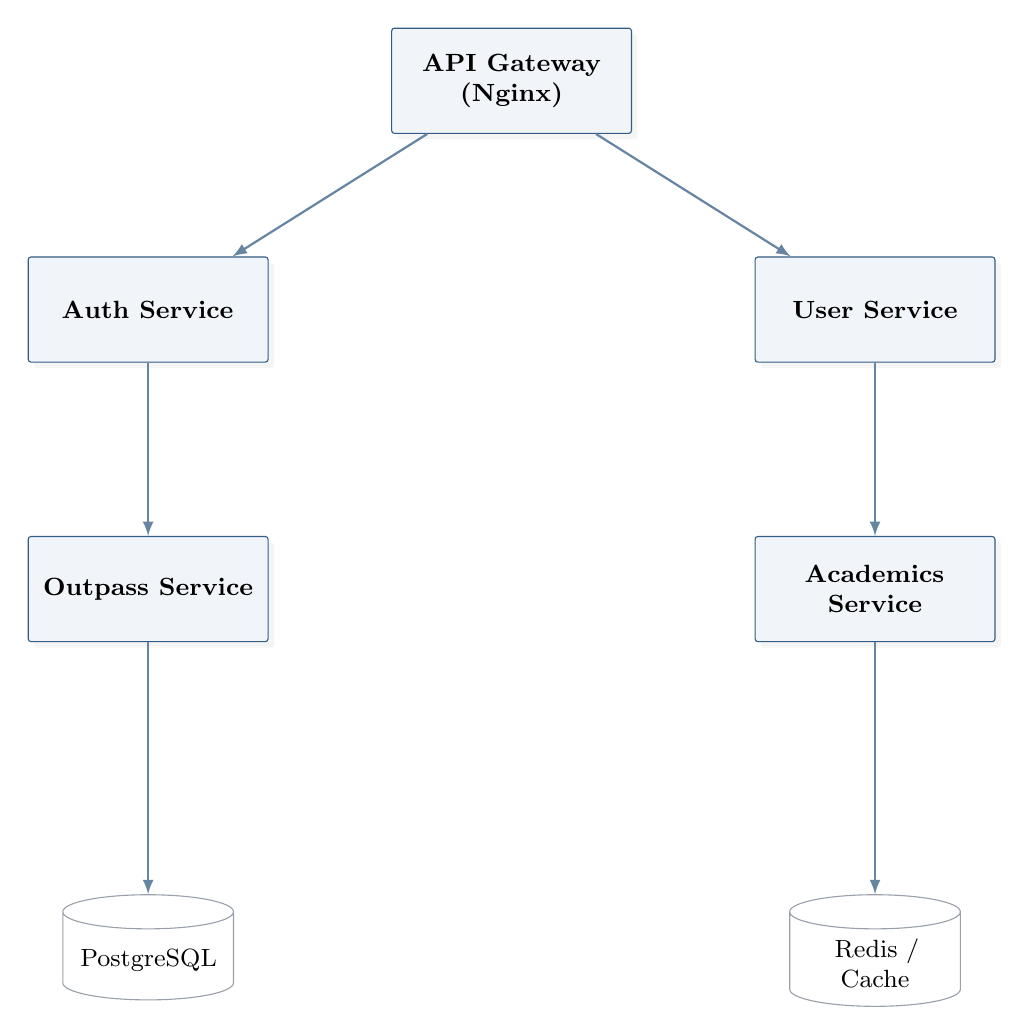
\begin{tikzpicture}[
    node distance=2.2cm,
    block/.style={rectangle, draw=unizblue!80, fill=unizlight, text width=8em, text centered, rounded corners=1pt, minimum height=3.8em, font=\bfseries\small, drop shadow={opacity=0.08}},
    db/.style={cylinder, draw=accent!50, fill=white, shape border rotate=90, aspect=0.2, text width=5.5em, text centered, minimum height=3.8em, font=\small},
    line/.style={draw, -latex, thick, color=unizblue!60}
]

% Nodes
\node [block] (gateway) {API Gateway\\(Nginx)};
\node [block, below left=of gateway] (auth) {Auth Service};
\node [block, below right=of gateway] (user) {User Service};
\node [block, below=of auth] (outpass) {Outpass Service};
\node [block, below=of user] (academics) {Academics Service};
\node [db, below=of outpass, yshift=-1cm] (db1) {PostgreSQL};
\node [db, below=of academics, yshift=-1cm] (db2) {Redis / Cache};

% Connectors
\path [line] (gateway) -- (auth);
\path [line] (gateway) -- (user);
\path [line] (auth) -- (outpass);
\path [line] (user) -- (academics);
\path [line] (outpass) -- (db1);
\path [line] (academics) -- (db2);

\end{tikzpicture}
\caption{System Component Relationship Mapping}
\end{figure}

\subsection{Approval Chain Logic}
\begin{figure}[h]
\centering
\begin{tikzpicture}[
    node distance=1.8cm,
    step/.style={rectangle, draw=accent!30, fill=white, text width=8.5em, text centered, minimum height=3.2em, rounded corners=0.5pt, font=\small, drop shadow={opacity=0.05}},
    arrow/.style={draw, -latex, thick, color=unizblue!40}
]

\node [step] (s1) {Student Submission};
\node [step, right=of s1] (s2) {Caretaker Review};
\node [step, right=of s2] (s3) {Warden Approval};
\node [step, right=of s3] (s4) {Dean / Director};

\draw [arrow] (s1) -- (s2);
\draw [arrow] (s2) -- (s3);
\draw [arrow] (s3) -- (s4);

\end{tikzpicture}
\caption{Multi-Tiered Approval Workflow}
\end{figure}

\subsection{Academic Grade Processing}
\begin{figure}[h]
\centering
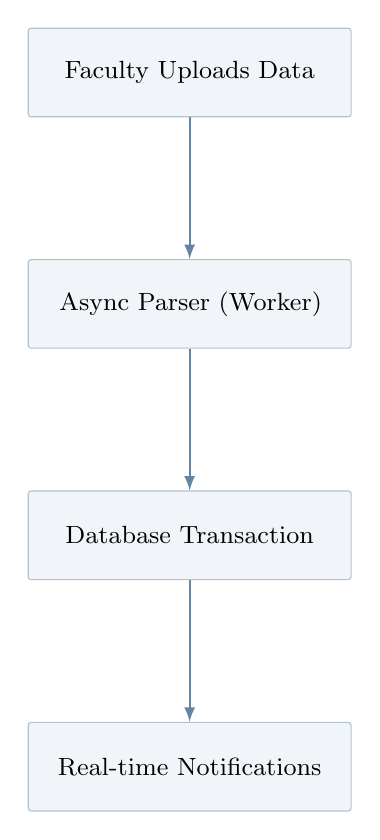
\begin{tikzpicture}[
    node distance=1.8cm,
    box/.style={rectangle, draw=unizblue!30, fill=unizlight, text width=11em, text centered, minimum height=3.2em, rounded corners=1pt, font=\small},
    arrow/.style={draw, -latex, thick, color=unizblue!60}
]

\node [box] (faculty) {Faculty Uploads Data};
\node [box, below=of faculty] (worker) {Async Parser (Worker)};
\node [box, below=of worker] (db) {Database Transaction};
\node [box, below=of db] (notify) {Real-time Notifications};

\draw [arrow] (faculty) -- (worker);
\draw [arrow] (worker) -- (db);
\draw [arrow] (db) -- (notify);

\end{tikzpicture}
\caption{Data Ingestion Pipeline}
\end{figure}

\subsection{Authentication Sequence}
\begin{figure}[h]
\centering
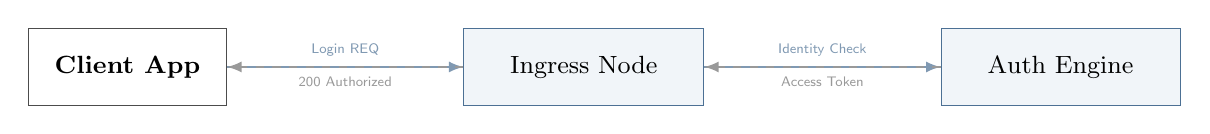
\begin{tikzpicture}[
    node distance=3cm,
    actor/.style={rectangle, draw=black!70, fill=white, text width=6.5em, text centered, minimum height=2.8em, font=\bfseries\small},
    svc/.style={rectangle, draw=unizblue!70, fill=unizlight, text width=8em, text centered, minimum height=2.8em, font=\small},
    arrow/.style={draw, -latex, thick, color=unizblue!50}
]

\node [actor] (user) {Client App};
\node [svc, right=of user] (gateway) {Ingress Node};
\node [svc, right=of gateway] (auth) {Auth Engine};

\draw [arrow] (user.east) -- node[above, font=\tiny\sffamily] {Login REQ} (gateway.west);
\draw [arrow] (gateway.east) -- node[above, font=\tiny\sffamily] {Identity Check} (auth.west);
\draw [arrow, dashed, color=gray!80] (auth.west) -- node[below, font=\tiny\sffamily] {Access Token} (gateway.east);
\draw [arrow, dashed, color=gray!80] (gateway.west) -- node[below, font=\tiny\sffamily] {200 Authorized} (user.east);

\end{tikzpicture}
\caption{Internal Identity Negotiation Flow}
\end{figure}

\section{Technical Implementation}
\subsection{Uniz Portal}
\subsubsection*{apps/uniz-portal/vite.config.ts}
\begin{lstlisting}
import { defineConfig } from "vite";
import react from "@vitejs/plugin-react";
import path from "path";
import { fileURLToPath } from "url";

const __filename = fileURLToPath(import.meta.url);
const __dirname = path.dirname(__filename);

// https://vitejs.dev/config/
export default defineConfig({
  plugins: [react()],
  resolve: {
    alias: {
      "@": path.resolve(__dirname, "./src"),
    },
  },
  server: {
    proxy: {
      "/api": {
        target: "https://api.uniz.rguktong.in",
        changeOrigin: true,
        secure: true,
      },
    },
  },
});

\end{lstlisting}
\subsubsection*{apps/uniz-portal/src/vite-env.d.ts}
\begin{lstlisting}
/// <reference types="vite/client" />

\end{lstlisting}
\subsubsection*{apps/uniz-portal/src/types/index.ts}
\begin{lstlisting}
// Interfaces

export interface Subject {
  id: string;
  name: string;
  credits: number;
}

export interface Semester {
  id: string;
  name: string;
  year: string;
}

export interface Grade {
  id: string;
  subjectId: string;
  grade: number;
  isRemedial?: boolean;
  subject: Subject;
  semester: Semester;
}

export interface Attendance {
  id: string;
  subjectId: string;
  totalClasses: number;
  attendedClasses: number;
  subject: Subject;
  semester: Semester;
}

export interface Outing {
  _id: string;
  from_time: string;
  to_time: string;
  in_time: string;
  reason: string;
  requested_time: string;
  is_approved: boolean;
  is_rejected: boolean;
  is_expired: boolean;
  issued_by?: string;
  issued_time?: string;
  rejected_by?: string;
  rejected_time?: string;
  message?: string;
  no_of_days: number;
}

export interface Outpass {
  _id: string;
  from_day: string;
  to_day: string;
  in_time: string;
  reason: string;
  requested_time: string;
  is_approved: boolean;
  is_rejected: boolean;
  is_expired: boolean;
  issued_by?: string;
  issued_time?: string;
  rejected_by?: string;
  rejected_time?: string;
  message?: string;
  no_of_days: number;
}

export interface Student {
  _id: string; // usually the username/id
  username: string;
  name: string;
  email: string;
  gender: string;
  year: string;
  branch: string;
  section: string;
  roomno: string;
  has_pending_requests: boolean;
  is_in_campus: boolean;

  // Academic
  grades: Grade[];
  attendance: Attendance[];

  // Personal
  blood_group: string;
  phone_number: string;
  date_of_birth: string;
  address?: string;

  // Parents
  father_name: string;
  father_phonenumber: string;
  father_email?: string;
  mother_name: string;
  mother_phonenumber: string;
  mother_email?: string;

  // History
  outings_list: Outing[];
  outpasses_list: Outpass[];

  profile_url?: string;

  created_at: string;
  updated_at: string;
}

export interface Faculty {
  id: string;
  Username: string;
  Name: string;
  Email: string;
  Department: string;
  Designation: string;
  Role: "teacher" | "hod";
  Contact: string;
  ProfileUrl?: string;
  subjects?: {
    subject: Subject;
  }[];
}

\end{lstlisting}
\subsubsection*{apps/uniz-portal/src/constants/developers.ts}
\begin{lstlisting}
export const developers = [
    {
        id: 1,
        name: "Sree Charan",
        designation: "Backend and Architecture",
        image: "https://res.cloudinary.com/diipfzmyj/image/upload/v1773549659/WhatsApp_Image_2026-01-25_at_20.21.46-modified_e6gcxw.png",
        url: "https://sreecharan.rguktong.in/",
    },
    {
        id: 2,
        name: "Bhanu Prakash",
        designation: "FrontEnd and UI",
        image: "https://res.cloudinary.com/diipfzmyj/image/upload/v1773550064/1000184711-modified_zmotfe.png",
        url: "https://bhanu-prakash.rguktong.in/",
    },
    {
        id: 3,
        name: "SitaRam",
        designation: "Security",
        image: "https://res.cloudinary.com/diipfzmyj/image/upload/v1773549648/sita-modified_lw9ulf.png",
        url: "https://seetharam.rguktong.in/",
    },
    {
        id: 4,
        name: "Anand",
        designation: "AI and Backend",
        image: "https://res.cloudinary.com/diipfzmyj/image/upload/v1773549648/anand-modified_lx5yvi.png",
        url: "https://anand-velpuri.rguktong.in/",
    },
];

\end{lstlisting}
\subsubsection*{apps/uniz-portal/src/utils/toast-ref.ts}
\begin{lstlisting}
import { ToasterProps, ToasterRef } from "@/components/ui/toast";
import { createRef } from "react";

export const toasterRef = createRef<ToasterRef>();

export const toast = {
  show: (props: ToasterProps) => {
    toasterRef.current?.show(props);
  },
  success: (message: string, optionsOrTitle?: string | Partial<ToasterProps>) => {
    const props: ToasterProps = typeof optionsOrTitle === 'object' 
      ? { message, variant: 'success', ...optionsOrTitle }
      : { message, title: optionsOrTitle, variant: 'success' };
    toasterRef.current?.show(props);
  },
  error: (message: string, optionsOrTitle?: string | Partial<ToasterProps>) => {
    const props: ToasterProps = typeof optionsOrTitle === 'object' 
      ? { message, variant: 'error', ...optionsOrTitle }
      : { message, title: optionsOrTitle, variant: 'error' };
    toasterRef.current?.show(props);
  },
  warning: (message: string, optionsOrTitle?: string | Partial<ToasterProps>) => {
    const props: ToasterProps = typeof optionsOrTitle === 'object' 
      ? { message, variant: 'warning', ...optionsOrTitle }
      : { message, title: optionsOrTitle, variant: 'warning' };
    toasterRef.current?.show(props);
  },
  info: (message: string, optionsOrTitle?: string | Partial<ToasterProps>) => {
    const props: ToasterProps = typeof optionsOrTitle === 'object' 
      ? { message, variant: 'default', ...optionsOrTitle }
      : { message, title: optionsOrTitle, variant: 'default' };
    toasterRef.current?.show(props);
  },
};

\end{lstlisting}
\subsubsection*{apps/uniz-portal/src/utils/timeUtils.ts}
\begin{lstlisting}
export const formatDateTime = (
  dateTimeString: string | undefined | null,
): string => {
  if (!dateTimeString) return "N/A";

  try {
    const date = new Date(dateTimeString);

    // Check if date is valid
    if (isNaN(date.getTime())) {
      return "Invalid Date";
    }

    const options: Intl.DateTimeFormatOptions = {
      timeZone: "Asia/Kolkata",
      day: "2-digit",
      month: "2-digit",
      year: "numeric",
      hour: "2-digit",
      minute: "2-digit",
      hour12: true,
    };

    return new Intl.DateTimeFormat("en-IN", options).format(date);
  } catch (error) {
    console.error("Error formatting date:", error);
    return "Invalid Date";
  }
};

// Optional: Add specific formatters for different use cases
export const formatDate = (dateString: string | undefined | null): string => {
  if (!dateString) return "N/A";

  try {
    const date = new Date(dateString);

    if (isNaN(date.getTime())) {
      return "Invalid Date";
    }

    return new Intl.DateTimeFormat("en-IN", {
      timeZone: "Asia/Kolkata",
      day: "2-digit",
      month: "2-digit",
      year: "numeric",
    }).format(date);
  } catch (error) {
    console.error("Error formatting date:", error);
    return "Invalid Date";
  }
};

export const formatTime = (timeString: string | undefined | null): string => {
  if (!timeString) return "N/A";

  try {
    const date = new Date(timeString);

    if (isNaN(date.getTime())) {
      return "Invalid Time";
    }

    return new Intl.DateTimeFormat("en-IN", {
      timeZone: "Asia/Kolkata",
      hour: "2-digit",
      minute: "2-digit",
      hour12: true,
    }).format(date);
  } catch (error) {
    console.error("Error formatting time:", error);
    return "Invalid Time";
  }
};

interface Duration {
  days: number | string;
  hours: number | string;
  minutes: number | string;
  seconds: number | string;
}

export const calculateDuration = (
  startTime: string,
  endTime: string,
): Duration => {
  try {
    // Handle empty or invalid inputs
    if (!startTime || !endTime) {
      return { days: "NaN", hours: "NaN", minutes: "NaN", seconds: "NaN" };
    }

    // For time-only strings (outings)
    if (!startTime.includes("/") && !endTime.includes("/")) {
      const parseTime = (timeStr: string) => {
        const lowerStr = timeStr.toLowerCase().trim();
        let hours = 0,
          minutes = 0,
          seconds = 0;

        if (lowerStr.includes("am") || lowerStr.includes("pm")) {
          const [time, meridiem] = lowerStr.split(" ");
          const [h, m, s = 0] = time.split(":").map(Number);
          hours = h;
          minutes = m;
          seconds = s;
          if (meridiem === "pm" && hours !== 12) hours += 12;
          else if (meridiem === "am" && hours === 12) hours = 0;
        } else {
          const [h, m, s = 0] = lowerStr.split(":").map(Number);
          hours = h;
          minutes = m;
          seconds = s;
        }
        return hours * 3600 + minutes * 60 + seconds;
      };

      const startSeconds = parseTime(startTime);
      const endSeconds = parseTime(endTime);
      const diffInSeconds = Math.abs(endSeconds - startSeconds);

      return {
        days: 0,
        hours: Math.floor(diffInSeconds / 3600),
        minutes: Math.floor((diffInSeconds % 3600) / 60),
        seconds: diffInSeconds % 60,
      };
    }

    // For full dates (outpasses)
    // Parse DD/MM/YYYY format
    const [startDay, startMonth, startYear] = startTime.split("/").map(Number);
    const [endDay, endMonth, endYear] = endTime.split("/").map(Number);

    const start = new Date(startYear, startMonth - 1, startDay);
    const end = new Date(endYear, endMonth - 1, endDay);

    if (isNaN(start.getTime()) || isNaN(end.getTime())) {
      return { days: "NaN", hours: "NaN", minutes: "NaN", seconds: "NaN" };
    }

    const diffInMilliseconds = end.getTime() - start.getTime();
    const diffInSeconds = diffInMilliseconds / 1000;

    return {
      days: Math.floor(diffInSeconds / (24 * 3600)),
      hours: Math.floor((diffInSeconds % (24 * 3600)) / 3600),
      minutes: Math.floor((diffInSeconds % 3600) / 60),
      seconds: Math.floor(diffInSeconds % 60),
    };

\end{lstlisting}
\subsubsection*{apps/uniz-portal/src/utils/academicCache.ts}
\begin{lstlisting}
/**
 * academicCache.ts
 * ─────────────────────────────────────────────────────────────────
 * Shared localStorage cache for academic data (grades & attendance).
 *
 * Cache key format: uniz_academic_{type}_{userId}_{year}_{semester}
 * TTL: 30 minutes - data is stale-while-revalidate after this.
 * ─────────────────────────────────────────────────────────────────
 */

const CACHE_TTL_MS = 30 * 60 * 1000; // 30 minutes

type CacheType = "grades" | "attendance";

function buildKey(
  type: CacheType,
  userId: string,
  year: string,
  semester: string,
): string {
  return `uniz_academic_${type}_${userId}_${year}_${semester}`;
}

export interface CacheEntry<T> {
  data: T;
  timestamp: number;
}

/** Write a result to cache */
export function writeAcademicCache<T>(
  type: CacheType,
  userId: string,
  year: string,
  semester: string,
  data: T,
): void {
  try {
    const entry: CacheEntry<T> = { data, timestamp: Date.now() };
    localStorage.setItem(
      buildKey(type, userId, year, semester),
      JSON.stringify(entry),
    );
  } catch {
    // Quota exceeded - silently skip
  }
}

/** Read a result from cache. Returns null if missing or expired. */
export function readAcademicCache<T>(
  type: CacheType,
  userId: string,
  year: string,
  semester: string,
  allowStale = false,
): T | null {
  try {
    const raw = localStorage.getItem(buildKey(type, userId, year, semester));
    if (!raw) return null;
    const entry: CacheEntry<T> = JSON.parse(raw);
    if (!allowStale && Date.now() - entry.timestamp > CACHE_TTL_MS) {
      // Expired - remove it
      localStorage.removeItem(buildKey(type, userId, year, semester));
      return null;
    }
    return entry.data;
  } catch {
    return null;
  }
}

/** Check if a cache entry is stale (older than TTL) without removing it */
export function isCacheStale(
  type: CacheType,
  userId: string,
  year: string,
  semester: string,
): boolean {
  try {
    const raw = localStorage.getItem(buildKey(type, userId, year, semester));
    if (!raw) return true;
    const entry: CacheEntry<unknown> = JSON.parse(raw);
    return Date.now() - entry.timestamp > CACHE_TTL_MS;
  } catch {
    return true;
  }
}

/** Clear all academic cache entries for a specific user */
export function clearAcademicCache(userId: string): void {
  try {
    const keysToRemove: string[] = [];
    for (let i = 0; i < localStorage.length; i++) {
      const key = localStorage.key(i);
      if (key && key.startsWith(`uniz_academic_`) && key.includes(userId)) {
        keysToRemove.push(key);
      }
    }
    keysToRemove.forEach((k) => localStorage.removeItem(k));
  } catch {
    // ignore
  }
}

\end{lstlisting}
\subsubsection*{apps/uniz-portal/src/utils/polling.ts}
\begin{lstlisting}
// utils/polling.ts
export const pollProgress = async (
  url: string,
  token: string,
  onUpdate: (data: any) => void,
  onComplete: () => void,
) => {
  const interval = setInterval(async () => {
    try {
      const res = await fetch(url, {
        headers: { Authorization: `Bearer ${(token || "").replace(/"/g, "")}` },
      });
      const data = await res.json();
      if (data.success) {
        onUpdate(data);
        if (data.status === "completed" || data.status === "failed") {
          clearInterval(interval);
          onComplete();
        }
      } else {
        clearInterval(interval);
      }
    } catch {
      clearInterval(interval);
    }
  }, 3000);
};

\end{lstlisting}

\subsection{Uniz Academics}
\subsubsection*{apps/uniz-academics/verify-remedial-flow.ts}
\begin{lstlisting}
import { PrismaClient } from "@prisma/client";
import ExcelJS from "exceljs";
import { mapGradeToPoint } from "./src/utils/helpers.util";

const prisma = new PrismaClient({
  datasources: {
    db: {
      url: process.env.DATABASE_URL,
    },
  },
});

async function processExcel(filePath: string) {
  const workbook = new ExcelJS.Workbook();
  await workbook.xlsx.readFile(filePath);
  const worksheet = workbook.getWorksheet(1);
  if (!worksheet) return;

  const rows: any[] = [];
  const headers: string[] = [];
  worksheet.getRow(1).eachCell((cell) => {
    headers.push(String(cell.value).trim());
  });

  worksheet.eachRow((row, rowNumber) => {
    if (rowNumber === 1) return;
    const rowData: any = {};
    row.eachCell((cell, colNumber) => {
      rowData[headers[colNumber - 1]] = cell.value;
    });
    rows.push(rowData);
  });

  const allSubjects = await prisma.subject.findMany();
  const subjectMap = new Map(allSubjects.map((s) => [s.code, s]));

  console.log(`Processing ${rows.length} rows...`);

  for (const row of rows) {
    const studentId = String(row["Student ID"] || "")
      .toUpperCase()
      .trim();
    if (studentId !== "O210008") continue; // Only process the target student for test speed

    const code = String(row["Subject Code"] || "")
      .toUpperCase()
      .trim();
    const rawGrade = String(row["Grade (EX, A, B, C, D, E, R)"] || "").trim();
    const semesterId = String(row["Semester ID"] || "").trim();

    const subject = subjectMap.get(code);
    if (!subject) continue;

    const grade = mapGradeToPoint(rawGrade);
    const batchYear = studentId.substring(0, 3);

    const existingGrade = await prisma.grade.findUnique({
      where: {
        studentId_subjectId_semesterId: {
          studentId,
          subjectId: subject.id,
          semesterId,
        },
      },
    });

    let isRemedial = existingGrade?.isRemedial || false;
    if (existingGrade && existingGrade.grade === 0 && grade !== 0) {
      isRemedial = true;
      console.log(
        `[PASS] Student ${studentId} passed remedial for ${code}! Marking as isRemedial.`,
      );
    }

    await prisma.grade.upsert({
      where: {
        studentId_subjectId_semesterId: {
          studentId,
          subjectId: subject.id,
          semesterId,
        },
      },
      update: { grade, batch: batchYear, isRemedial, updatedAt: new Date() },
      create: {
        studentId,
        subjectId: subject.id,
        semesterId,
        grade,
        batch: batchYear,
        isRemedial,
      },
    });
  }
}

const filePath =
  "/Users/sreecharandesu/Projects/uniz-master/tests/data/grades_upload/O21_E4_SEM-2.xlsx";

processExcel(filePath)
  .then(() => console.log("Processing finished."))
  .catch(console.error)
  .finally(() => prisma.$disconnect());

\end{lstlisting}
\subsubsection*{apps/uniz-academics/check-db.ts}
\begin{lstlisting}
import { PrismaClient } from "@prisma/client";
const prisma = new PrismaClient();

async function main() {
  const semesters = await prisma.academicSemester.findMany();
  console.log("Semesters:", semesters);

  const allocations = await prisma.branchAllocation.findMany({
    include: { subject: true },
  });
  console.log("Allocations count:", allocations.length);
  const cseAllocations = allocations.filter((a) => a.branch === "CSE");
  console.log(
    "CSE Allocations:",
    cseAllocations.map((a) => ({
      code: a.subject.code,
      approved: a.isApproved,
    })),
  );
}

main()
  .catch(console.error)
  .finally(() => prisma.$disconnect());

\end{lstlisting}
\subsubsection*{apps/uniz-academics/test\_env.ts}
\begin{lstlisting}
import dotenv from 'dotenv';
import path from 'path';

dotenv.config();

console.log('--- Academics Env Debug ---');
console.log('JWT_SECURITY_KEY:', process.env.JWT_SECURITY_KEY);
console.log('INTERNAL_SECRET:', process.env.INTERNAL_SECRET);
console.log('AUTH_SERVICE_URL:', process.env.AUTH_SERVICE_URL);
console.log('DATABASE_URL:', process.env.DATABASE_URL);
console.log('--- End ---');

\end{lstlisting}
\subsubsection*{apps/uniz-academics/test-remedial.ts}
\begin{lstlisting}
import { PrismaClient } from "@prisma/client";
import { mapGradeToPoint } from "./src/utils/helpers.util";

const prisma = new PrismaClient({
  datasources: {
    db: {
      url: process.env.DATABASE_URL,
    },
  },
});

async function testRemedial() {
  const studentId = "TEST_STUDENT_001";
  const subjectCode = "CSE-E1-SEM-1-01";
  const semesterId = "SEM-1";

  console.log("--- Testing Remedial Logic ---");

  // 1. Get subject
  const subject = await prisma.subject.findUnique({
    where: { code: subjectCode },
  });
  if (!subject) {
    console.error("Subject not found!");
    return;
  }

  // 2. Clear existing test data
  await prisma.grade.deleteMany({
    where: { studentId, subjectId: subject.id, semesterId },
  });

  console.log("Stage 1: Inserting initial FAIL (R)");
  // Simulate first upload: Student fails
  const initialGrade = 0; // 'R'
  await prisma.grade.create({
    data: {
      studentId,
      subjectId: subject.id,
      semesterId,
      grade: initialGrade,
      batch: "O21",
      isRemedial: false,
    },
  });

  let gradeRec = await prisma.grade.findUnique({
    where: {
      studentId_subjectId_semesterId: {
        studentId,
        subjectId: subject.id,
        semesterId,
      },
    },
  });
  console.log("Initial Record:", gradeRec);

  console.log("\nStage 2: Uploading Remedial PASS (EX)");
  // Simulate second upload: Student passes remedial
  const newGrade = 10; // 'EX'

  // Logic from upload.service.ts
  const existingGrade = await prisma.grade.findUnique({
    where: {
      studentId_subjectId_semesterId: {
        studentId,
        subjectId: subject.id,
        semesterId,
      },
    },
  });

  let isRemedial = existingGrade?.isRemedial || false;
  if (existingGrade && existingGrade.grade === 0 && newGrade !== 0) {
    isRemedial = true;
  }

  await prisma.grade.upsert({
    where: {
      studentId_subjectId_semesterId: {
        studentId,
        subjectId: subject.id,
        semesterId,
      },
    },
    update: { grade: newGrade, isRemedial, updatedAt: new Date() },
    create: {
      studentId,
      subjectId: subject.id,
      semesterId,
      grade: newGrade,
      isRemedial,
    },
  });

  gradeRec = await prisma.grade.findUnique({
    where: {
      studentId_subjectId_semesterId: {
        studentId,
        subjectId: subject.id,
        semesterId,
      },
    },
  });
  console.log("Updated Record (Should be Remedial):", gradeRec);

  if (gradeRec?.isRemedial === true) {
    console.log("\n✅ SUCCESS: Record marked as remedial!");
  } else {
    console.log("\n❌ FAILURE: Record NOT marked as remedial.");
  }

  // Cleanup
  // await prisma.grade.deleteMany({ where: { studentId } });
}

testRemedial()
  .catch(console.error)
  .finally(() => prisma.$disconnect());

\end{lstlisting}
\subsubsection*{apps/uniz-academics/prisma/schema.prisma}
\begin{lstlisting}
generator client {
  provider = "prisma-client-js"
  binaryTargets = ["native", "rhel-openssl-3.0.x", "linux-musl-arm64-openssl-3.0.x"]
}

datasource db {
  provider = "postgresql"
  url      = env("DATABASE_URL")
}

model Subject {
  id                String             @id
  code              String             @unique
  name              String
  credits           Float
  department        String
  semester          String
  attendance        Attendance[]
  grades            Grade[]
  branchAllocations   BranchAllocation[]
  registrations       Registration[]
  seatingArrangements SeatingArrangement[]
}

model Grade {
  id            String   @id @default(uuid()) @db.Uuid
  studentId     String
  subjectId     String
  semesterId    String
  attemptNumber Int      @default(1)
  grade         Float
  batch         String? // e.g. "O21"
  isRemedial    Boolean  @default(false)
  passDate            DateTime?
  subjectNameOverride String? // For electives (e.g. "Cloud Computing" instead of "Elective-VI")
  createdAt           DateTime @default(now())
  updatedAt           DateTime @updatedAt
  subject             Subject  @relation(fields: [subjectId], references: [id])

  @@unique([studentId, subjectId, semesterId, attemptNumber])
  @@index([studentId])
  @@index([batch])
  @@index([semesterId])
}

model Attendance {
  id              String   @id @default(uuid()) @db.Uuid
  studentId       String
  subjectId       String
  semesterId      String
  totalClasses    Int
  attendedClasses Int
  batch           String? // e.g. "O21"
  subjectNameOverride String? // For electives (e.g. "Cloud Computing" instead of "Elective-VI")
  createdAt       DateTime @default(now())
  updatedAt       DateTime @updatedAt
  subject         Subject  @relation(fields: [subjectId], references: [id])

  @@unique([studentId, subjectId, semesterId])
  @@index([studentId])
  @@index([batch])
  @@index([semesterId])
}

enum SemesterStatus {
  DRAFT
  DEAN_REVIEW
  APPROVED
  REGISTRATION_OPEN
  REGISTRATION_CLOSED
}

model AcademicSemester {
  id                String             @id
  name              String // e.g. "AY 2024-25 SEM-II"
  status            SemesterStatus     @default(DRAFT)
  branchAllocations   BranchAllocation[]
  registrations       Registration[]
  seatingArrangements SeatingArrangement[]
  createdAt           DateTime           @default(now())
  updatedAt         DateTime           @updatedAt
}

model Faculty {
  id          String   @id @default(uuid()) @db.Uuid
  name        String
  email       String   @unique
  photo       String?
  department  String
  designation String?  @default("Assistant Professor")
  role        String   @default("FACULTY") // "FACULTY", "HOD", "DEAN", "WEBMASTER"
  bio         Json?
  createdAt   DateTime @default(now())
  updatedAt   DateTime @updatedAt

  @@index([department])
}

enum AllocationStatus {
  DEAN_PENDING
  HOD_REVIEW
  APPROVED
}

model BranchAllocation {
  id            String           @id @default(uuid()) @db.Uuid
  branch        String // e.g. "CSE", "ECE"
  academicYear  String?          @default("E1") // e.g. "E1", "E2", "E3", "E4"
  batch         String?          @default("")   // e.g. "O21"
  subjectId     String
  semesterId    String
  customName    String? // For electives (e.g. ELECTIVE (NPTEL Course))
  customCredits Int? // Ability to override default subject credits
  status        AllocationStatus @default(DEAN_PENDING)
  isApproved    Boolean          @default(false)
  isMandatory   Boolean          @default(true)
  electiveGroupId String?        @default("")
  electiveLimit Int?             @default(1)
  subject       Subject          @relation(fields: [subjectId], references: [id])
  semester      AcademicSemester @relation(fields: [semesterId], references: [id])

  @@unique([branch, subjectId, semesterId])
  @@index([branch])
  @@index([semesterId])
  @@index([academicYear])
  @@index([batch])
}

model Registration {
  id         String           @id @default(uuid()) @db.Uuid
  studentId  String
  batch      String?          @default("") // e.g. "O21"
  subjectId  String
  semesterId String
  status     String           @default("REGISTERED") // "REGISTERED", "DROPPED"
  subject    Subject          @relation(fields: [subjectId], references: [id])
  semester   AcademicSemester @relation(fields: [semesterId], references: [id])
  createdAt  DateTime         @default(now())
  updatedAt  DateTime         @updatedAt

  @@unique([studentId, subjectId, semesterId])
  @@index([studentId])
  @@index([semesterId])
  @@index([batch])
}

model SeatingArrangement {
  id         String           @id @default(uuid()) @db.Uuid
  studentId  String
  batch      String?          @default("") // e.g. "O21"

\end{lstlisting}
\subsubsection*{apps/uniz-academics/prisma/safe\_seed.ts}
\begin{lstlisting}
import { PrismaClient } from "@prisma/client";

const prisma = new PrismaClient();

const subjectsData: any = {
  E1: {
    "Sem - 1": {
      CSE: {
        names: [
          "Calculus & Linear Algebra",
          "Basic Electrical and Electronics Engg.",
          "Problem Solving and Programming Through C",
          "Engineering Graphics & Computer Drafting",
          "English-Language communication Skills Lab-I",
          "Basic Electrical and Electronics Engg. Lab",
          "Problem Solving and Programming Through C Lab",
        ],
        credits: [4, 4, 4, 2.5, 2.5, 1.5, 1.5],
      },
      ECE: {
        names: [
          "Differential Equations and Multivariable Calculus",
          "Engineering Physics",
          "Engineering Physics Lab",
          "Engineering Graphics and Design",
          "Electrical Technology",
          "Electrical Technology Lab",
          "Introduction to Latest Technical Advancements",
          "Programming & Data Structures",
          "Programming & Data Structures Lab",
          "Biology for Engineers",
        ],
        credits: [4, 4, 1.5, 2.5, 4, 1.5, 1, 3, 1.5, 0],
      },
      EEE: {
        names: [
          "Differential Equations and Multivariable calculus",
          "Engineering Physics",
          "Engineering Physics Lab",
          "Engineering Graphics & Computer Drafting",
          "Electrical Technology",
          "Electrical Technology Lab",
          "Introduction to Latest Technical Advancements",
          "Programming & Data Structures",
          "Programming & Data Structures Lab",
        ],
        credits: [4, 4, 1.5, 2.5, 4, 1.5, 1, 3, 1.5, 0],
      },
      CIVIL: {
        names: [
          "Engineering Chemistry",
          "Differential Equations and Multivariable Calculus",
          "Basic Programming Language",
          "Engineering Graphics and Computer Drafting",
          "Computer Aided Drafting (CAD) Lab",
          "English Language Communication Skills Lab-I",
          "C Programming Lab",
          "Human Values",
        ],
        credits: [3, 4, 4, 2.5, 1.5, 2.5, 1.5, 0],
      },
      MECH: {
        names: [
          "Differential Equations and Multivariable Calculus",
          "English Language Communication Skills Lab - 1",
          "Engineering Physics",
          "Basic Electrical and Electronics Engineering",
          "Engineering Chemistry",
          "Workshop Practice",
          "Basic Electrical & Electronics Engineering Lab",
          "Engineering Physics & Chemistry Lab",
        ],
        credits: [4, 2.5, 4, 4, 3, 1.5, 1.5, 1.5],
      },
    },
    "Sem - 2": {
      CSE: {
        names: [
          "Discrete Mathematics",
          "Engineering Physics",
          "Managerial Economics and Finance Analysis",
          "Object Oriented Programming through Java",
          "Data Structures",
          "Engineering Physics Lab",
          "Object Oriented Programming through Java Lab",
          "Data Structures Lab",
        ],
        credits: [4, 4, 3, 4, 3, 1.5, 1.5, 1.5],
      },
      ECE: {
        names: [
          "Mathematical Methods",
          "Object Oriented Programming",
          "Object Oriented Programming Laboratory",
          "Computational Lab",
          "English-Language Communication Skills Lab-1",
          "Electronic Devices and Circuits",
          "Electronic Devices and Circuits Lab",
          "Network Theory",
          "Signals and Systems",
        ],
        credits: [4, 2, 1.5, 1.5, 2.5, 4, 1.5, 4, 4],
      },
      EEE: {
        names: [
          "Linear Algebra & Numerical Methods",
          "Digital Logic Design",
          "Digital Logic Design Lab",
          "Computational Lab",
          "English Language communication skills lab 1",
          "Electronic Devices and Circuits",
          "Electronic Devices and Circuits Lab",
          "Network Theory",
          "Introduction to AI",
        ],
        credits: [4, 4, 1.5, 1.5, 2.5, 4, 1.5, 4, 1],
      },
      CIVIL: {
        names: [
          "Advanced Programming Course",
          "Linear Algebra and Numerical Methods",
          "Basic Electrical and Electronics Engineering",
          "Engineering Mechanics",
          "Engineering Geology",
          "Advanced Programming Lab",
          "Workshop",
          "Environmental Science",
        ],
        credits: [3, 4, 3, 4, 3, 1.5, 1.5, 0],
      },
      MECH: {
        names: [
          "Mathematical Methods",
          "Engineering Mechanics",
          "Material Science & Metallurgy",
          "Programming and Data Structures",
          "Engineering Graphics and Computer Drafting",
          "Programming and Data Structures Lab",
          "Material Science and Metallurgy Lab",
        ],
        credits: [4, 4, 3, 3, 2.5, 1.5, 1.5],
      },
    },
  },
  E2: {
    "Sem - 1": {
      CSE: {
        names: [
          "Probability and Statistics",
          "Digital Logic Design",

\end{lstlisting}
\subsubsection*{apps/uniz-academics/prisma/seed.ts}
\begin{lstlisting}
import { PrismaClient } from "@prisma/client";
import * as fs from "fs";
import * as path from "path";

const prisma = new PrismaClient();

const subjectsData: any = {
  'E1': {
    'Sem - 1': {
      'CSE': {
        names: ["Calculus & Linear Algebra", "Basic Electrical and Electronics Engg.", "Problem Solving and Programming Through C", "Engineering Graphics & Computer Drafting", "English-Language communication Skills Lab-I", "Basic Electrical and Electronics Engg. Lab", "Problem Solving and Programming Through C Lab", "", ""],
        credits: [4, 4, 4, 2.5, 2.5, 1.5, 1.5, 0, 0, 0],
        hide: [8, 9]
      },
      'ECE': {
        names: ["Differential Equations and Multivariable Calculus", "Engineering Physics", "Engineering Physics Lab", "Engineering Graphics and Design", "Electrical Technology", "Electrical Technology Lab", "Introduction to Latest Technical Advancements", "Programming & Data Structures", "Programming & Data Structures Lab", "Biology for Engineers"],
        credits: [4, 4, 1.5, 2.5, 4, 1.5, 1, 3, 1.5, 0],
        hide: []
      },
      'EEE': {
        names: ["Differential Equations and Multivariable calculus", "Engineering Physics", "Engineering Physics Lab", "Engineering Graphics & Computer Drafting", "Electrical Technology", "Electrical Technology Lab", "Introduction to Latest Technical Advancements", "Programming & Data Structures", "Programming & Data Structures Lab"],
        credits: [4, 4, 1.5, 2.5, 4, 1.5, 1, 3, 1.5, 0]
      },
      'CIVIL': {
        names: ["Engineering Chemistry", "Differential Equations and Multivariable Calculus", "Basic Programming Language", "Engineering Graphics and Computer Drafting", "Computer Aided Drafting (CAD) Lab", "English Language Communication Skills Lab-I", "C Programming Lab", "Human Values", "", ""],
        credits: [3, 4, 4, 2.5, 1.5, 2.5, 1.5, 0, 0, 0],
        hide: [8, 9]
      },
      'MECH': {
        names: ["Differential Equations and Multivariable Calculus", "English Language Communication Skills Lab - 1", "Engineering Physics", "Basic Electrical and Electronics Engineering", "Engineering Chemistry", "Workshop Practice", "Basic Electrical & Electronics Engineering Lab", "Engineering Physics & Chemistry Lab", ""],
        credits: [4, 2.5, 4, 4, 3, 1.5, 1.5, 1.5, 0, 0],
        hide: [9]
      }
    },
    'Sem - 2': {
      'CSE': {
        names: ["Discrete Mathematics", "Engineering Physics", "Managerial Economics and Finance Analysis", "Object Oriented Programming through Java", "Data Structures", "Engineering Physics Lab", "Object Oriented Programming through Java Lab", "Data Structures Lab", ""],
        credits: [4, 4, 3, 4, 3, 1.5, 1.5, 1.5, 0, 0],
        hide: [9]
      },
      'ECE': {
        names: ["Mathematical Methods", "Object Oriented Programming", "Object Oriented Programming Laboratory", "Computational Lab", "English-Language Communication Skills Lab-1", "Electronic Devices and Circuits", "Electronic Devices and Circuits Lab", "Network Theory", "Signals and Systems", ""],
        credits: [4, 2, 1.5, 1.5, 2.5, 4, 1.5, 4, 4, 0],
        hide: [9]
      },
      'EEE': {
        names: ["Linear Algebra & Numerical Methods", "Digital Logic Design", "Digital Logic Design Lab", "Computational Lab", "English Language communication skills lab 1", "Electronic Devices and Circuits", "Electronic Devices and Circuits Lab", "Network Theory", "Introduction to AI"],
        credits: [4, 4, 1.5, 1.5, 2.5, 4, 1.5, 4, 1, 0]
      },
      'CIVIL': {
        names: ["Advanced Programming Course", "Linear Algebra and Numerical Methods", "Basic Electrical and Electronics Engineering", "Engineering Mechanics", "Engineering Geology", "Advanced Programming Lab", "Workshop", "Environmental Science", "", ""],
        credits: [3, 4, 3, 4, 3, 1.5, 1.5, 0, 0, 0],
        hide: [8, 9]
      },
      'MECH': {
        names: ["Mathematical Methods", "Engineering Mechanics", "Material Science & Metallurgy", "Programming and Data Structures", "Engineering Graphics and Computer Drafting", "Programming and Data Structures Lab", "Material Science and Metallurgy Lab", "", ""],
        credits: [4, 4, 3, 3, 2.5, 1.5, 1.5, 0, 0, 0],
        hide: [8, 9]
      }
    }
  },
  'E2': {
    'Sem - 1': {
      'CSE': {
        names: ["Probability and Statistics", "Digital Logic Design", "Design & Analysis of Algorithms", "Database Management Systems", "Formal Languages & Automata Theory", "Design & Analysis of Algorithms Lab", "Digital Logic Design Lab", "Database Management Systems Lab", ""],
        credits: [4, 3, 4, 3, 3, 1.5, 1.5, 1.5, 0, 0],
        hide: [9]
      },
      'ECE': {
        names: ["Probability & Random Variables", "Internet of Things Lab", "Analog Electronic Circuits", "Analog Electronic Circuits Lab", "Digital Logic Design", "Digital Logic Design Lab", "Digital Signal Processing", "Digital Signal Processing Lab", "Control Systems", ""],
        credits: [3, 1.5, 4, 1.5, 4, 1.5, 4, 1.5, 3, 0],
        hide: [9]
      },
      'EEE': {
        names: ["Probability & Random Variables", "Internet of Things Lab", "Analog Electronic Circuits", "Analog Electronic Circuits Lab", "Object Oriented Programming", "Object Oriented Programming Lab", "Signals & Systems", "Electrical Machines", "Electrical Machines Lab"],
        credits: [3, 1, 4, 1.5, 3, 1, 4, 4, 1.5, 0]
      },
      'CIVIL': {
        names: ["Management Economics and Financial Analysis", "Building Materials and Construction", "Concrete Technology", "Mechanics of Fluids", "Mechanics of Materials", "Surveying", "Mechanics of Materials Lab", "Surveying Lab", "Indian Constitution", ""],
        credits: [3, 3, 3, 3, 4, 4, 1.5, 1.5, 0, 0],
        hide: [9]
      },
      'MECH': {
        names: ["Transform Calculus", "Kinematics of Machinery", "Thermodynamics", "Mechanics of Solids", "Manufacturing Processes", "Mechanics of Solids Lab", "Computer Aided Machine Drawing", "", ""],
        credits: [4, 4, 4, 4, 3, 1.5, 1.5, 0, 0, 0],
        hide: [8, 9]
      }
    },
    'Sem - 2': {
      'CSE': {
        names: ["Introduction to Operation Research", "Computer Organization & Architecture", "Data Science with Python", "Web Technologies", "Compiler Design", "Computer Organization & Architecture Lab", "Data Science with Python Lab", "Web Technologies Lab", ""],
        credits: [3, 3, 3, 3, 3, 1.5, 1.5, 1.5, 0, 0],
        hide: [9]
      },
      'ECE': {
        names: ["Robotics Laboratory", "Communication Systems-1", "Communication Systems-1 Lab", "Digital System Design", "Digital System Design Lab", "Linear Integrated Circuits", "Linear Integrated Circuits Lab", "Electromagnetic Waves & Guided Media", "Foundations to Artificial Intelligence", ""],
        credits: [2.5, 4, 1.5, 3, 1.5, 4, 1.5, 4, 1, 0],
        hide: [9]
      },
      'EEE': {
        names: ["Robotics Laboratory", "Power Systems-I", "Machine Learning", "Control Systems", "Control Systems Lab", "Linear Integrated Circuits", "Linear Integrated Circuits Lab", "Power Electronics", "Power Electronics Lab"],
        credits: [1, 4, 3, 4, 1.5, 4, 1.5, 4, 1.5, 0]
      },
      'CIVIL': {
        names: ["Hydraulics Engineering", "Environmental Engineering-I", "Geo-Technical Engineering-I", "Structural Analysis", "Water Resources Engineering", "Introduction to Probability and Statistics", "Hydraulics Engineering Lab", "Geotechnical Engineering Lab", "", ""],
        credits: [3, 3, 4, 4, 3, 3, 1.5, 1.5, 0, 0],
        hide: [8, 9]
      },
      'MECH': {
        names: ["Design of Machine Elements", "Dynamics of Machinery", "Fluid Mechanics & Hydraulic Machinery", "Metal Cutting and Machine Tools", "Probability and Statistics", "Metal cutting and Machine Tools Lab", "Fluid Mechanics & Hydraulic Machinery Lab", "", ""],
        credits: [4, 4, 4, 4, 3, 1.5, 1.5, 0, 0, 0],
        hide: [8, 9]
      }
    }
  },
  'E3': {
    'Sem - 1': {
      'CSE': {
        names: ["Operating System", "Computer Networks", "Software Engineering", "Cloud Computing / Other Choosen", "Artificial Intelligence & Search methods", "Operating System Lab", "Computer Networks Lab", "Software Engineering Lab", "English-Language communication Skills Lab- II"],
        credits: [3, 3, 3, 3, 3, 1.5, 1.5, 1.5, 1.5, 0]
      },
      'ECE': {
        names: ["Computer Networks", "Computer Organization & Design based on RISC V", "English-Language Communication Skills Lab-2", "Communication Systems-2", "Communication Systems-2 Lab", "Microprocessors Lab", "Radio Frequency & Microwave Engg. Lab", "Mini-Project-I (Socially Relevant Project)", "Product Design & Innovation Lab", "RF & Microwave Engineering"],
        credits: [3, 3, 1.5, 4, 1.5, 1.5, 1.5, 1, 1, 2],
        hide: []
      },
      'EEE': {
        names: ["Digital Signal Processing", "Power Systems-II", "Power Systems Lab", "English Language Communication Skills Lab-2", "Electrical Vehicles", "Electrical Vehicles Lab", "Embedded Systems", "Embedded Systems Lab", "Mini-Project-I (Socially Relevant Project)", "Product Design & Innovation Lab"],
        credits: [3, 4, 1.5, 1.5, 3, 1.5, 3, 1.5, 1, 1],
        show: [10]
      },
      'CIVIL': {
        names: ["Advanced Structural Analysis", "Design of Reinforced Concrete Structures", "Environmental Engineering-II", "Geo-Technical Engineering-II", "English Language Communication Skills Lab-II", "Environmental Engineering Lab", "Concrete Technology Lab", "Computer Applications in Civil Engineering Lab", "Aptitude & Reasoning", ""],
        credits: [4, 4, 3, 3, 1.5, 1.5, 1.5, 1.5, 0, 0],
        hide: [9]
      },
      'MECH': {
        names: ["Heat Transfer", "Robotics & Automation", "Applied Thermodynamics", "Metrology and Mechanical Measurements", "Metrology and Mechanical Measurements Lab", "Heat Transfer Lab", "Applied Thermodynamics Lab", "English Language Communication Skills Lab-II", ""],
        credits: [4, 3, 4, 3, 1.5, 1.5, 1.5, 1.5, 0, 0],
        hide: [9]
      }
    },
    'Sem - 2': {
      'CSE': {
        names: ["Cryptography and Networks Security", "Artificial Intelligence", "Elective II", "Elective III", "Open Elective-I", "English-Language communication Skills Lab-I -III", "Mini Project", "", "Summer Internship"],
        credits: [4, 4, 3, 3, 3, 1.5, 3, 0, 3, 0],
        hide: [8]
      },
      'ECE': {
        names: ["English-Language Communication Skills Lab-3", "Indian Constitution", "Elective-1", "Elective-2", "Open Elective-1", "Open Elective-2", "Mini Project-II", "Career Development Course", "", ""],

\end{lstlisting}
\subsubsection*{apps/uniz-academics/scripts/seed-clean.ts}
\begin{lstlisting}
import { PrismaClient } from "@prisma/client";
const prisma = new PrismaClient();

const subjectsData: any = {
  E1: {
    "Sem - 1": {
      CSE: {
        names: [
          "Calculus & Linear Algebra",
          "Basic Electrical and Electronics Engg.",
          "Problem Solving and Programming Through C",
          "Engineering Graphics & Computer Drafting",
          "English-Language communication Skills Lab-I",
          "Basic Electrical and Electronics Engg. Lab",
          "Problem Solving and Programming Through C Lab",
        ],
        credits: [4, 4, 4, 2.5, 2.5, 1.5, 1.5],
      },
      ECE: {
        names: [
          "Differential Equations and Multivariable Calculus",
          "Engineering Physics",
          "Engineering Physics Lab",
          "Engineering Graphics and Design",
          "Electrical Technology",
          "Electrical Technology Lab",
          "Introduction to Latest Technical Advancements",
          "Programming & Data Structures",
          "Programming & Data Structures Lab",
          "Biology for Engineers",
        ],
        credits: [4, 4, 1.5, 2.5, 4, 1.5, 1, 3, 1.5, 0],
      },
      EEE: {
        names: [
          "Differential Equations and Multivariable calculus",
          "Engineering Physics",
          "Engineering Physics Lab",
          "Engineering Graphics & Computer Drafting",
          "Electrical Technology",
          "Electrical Technology Lab",
          "Introduction to Latest Technical Advancements",
          "Programming & Data Structures",
          "Programming & Data Structures Lab",
        ],
        credits: [4, 4, 1.5, 2.5, 4, 1.5, 1, 3, 1.5],
      },
      CIVIL: {
        names: [
          "Engineering Chemistry",
          "Differential Equations and Multivariable Calculus",
          "Basic Programming Language",
          "Engineering Graphics and Computer Drafting",
          "Computer Aided Drafting (CAD) Lab",
          "English Language Communication Skills Lab-I",
          "C Programming Lab",
          "Human Values",
        ],
        credits: [3, 4, 4, 2.5, 1.5, 2.5, 1.5, 0],
      },
      MECH: {
        names: [
          "Differential Equations and Multivariable Calculus",
          "English Language Communication Skills Lab - 1",
          "Engineering Physics",
          "Basic Electrical and Electronics Engineering",
          "Engineering Chemistry",
          "Workshop Practice",
          "Basic Electrical & Electronics Engineering Lab",
          "Engineering Physics & Chemistry Lab",
        ],
        credits: [4, 2.5, 4, 4, 3, 1.5, 1.5, 1.5],
      },
    },
    "Sem - 2": {
      CSE: {
        names: [
          "Discrete Mathematics",
          "Engineering Physics",
          "Managerial Economics and Finance Analysis",
          "Object Oriented Programming through Java",
          "Data Structures",
          "Engineering Physics Lab",
          "Object Oriented Programming through Java Lab",
          "Data Structures Lab",
        ],
        credits: [4, 4, 3, 4, 3, 1.5, 1.5, 1.5],
      },
      ECE: {
        names: [
          "Mathematical Methods",
          "Object Oriented Programming",
          "Object Oriented Programming Laboratory",
          "Computational Lab",
          "English-Language Communication Skills Lab-1",
          "Electronic Devices and Circuits",
          "Electronic Devices and Circuits Lab",
          "Network Theory",
          "Signals and Systems",
        ],
        credits: [4, 2, 1.5, 1.5, 2.5, 4, 1.5, 4, 4],
      },
      EEE: {
        names: [
          "Linear Algebra & Numerical Methods",
          "Digital Logic Design",
          "Digital Logic Design Lab",
          "Computational Lab",
          "English Language communication skills lab 1",
          "Electronic Devices and Circuits",
          "Electronic Devices and Circuits Lab",
          "Network Theory",
          "Introduction to AI",
        ],
        credits: [4, 4, 1.5, 1.5, 2.5, 4, 1.5, 4, 1],
      },
      CIVIL: {
        names: [
          "Advanced Programming Course",
          "Linear Algebra and Numerical Methods",
          "Basic Electrical and Electronics Engineering",
          "Engineering Mechanics",
          "Engineering Geology",
          "Advanced Programming Lab",
          "Workshop",
          "Environmental Science",
        ],
        credits: [3, 4, 3, 4, 3, 1.5, 1.5, 0],
      },
      MECH: {
        names: [
          "Mathematical Methods",
          "Engineering Mechanics",
          "Material Science & Metallurgy",
          "Programming and Data Structures",
          "Engineering Graphics and Computer Drafting",
          "Programming and Data Structures Lab",
          "Material Science and Metallurgy Lab",
        ],
        credits: [4, 4, 3, 3, 2.5, 1.5, 1.5],
      },
    },
  },
  E2: {
    "Sem - 1": {
      CSE: {
        names: [
          "Probability and Statistics",
          "Digital Logic Design",
          "Design & Analysis of Algorithms",

\end{lstlisting}

\subsection{Uniz Gateway}
\subsubsection*{apps/uniz-gateway/src/index.ts}
\begin{lstlisting}
import express from "express";
import cors from "cors";
import axios from "axios";
import path from "path";
import compression from "compression";
import Redis from "ioredis";
import httpProxy from "http-proxy";
import http from "http";
import dotenv from "dotenv";
dotenv.config({ override: true });

// Pre-configured Axios instance for internal communications with Keep-Alive
const internalClient = axios.create({
  timeout: 5000,
  httpAgent: new http.Agent({ keepAlive: true, maxSockets: 200 }),
});

const app = express();
app.set("trust proxy", 1);
const PORT = process.env.PORT || 3000;

// Initialize Redis for High-Speed Caching
const redis = new Redis(process.env.REDIS_URL || "redis://uniz-redis:6379", {
  maxRetriesPerRequest: 3,
  retryStrategy: (times: number) => Math.min(times * 50, 2000),
});

redis.on("error", (err: Error) =>
  console.error("[Redis] Connection Error:", err.message),
);
redis.on("connect", () => console.log("[Redis] Connected for Caching"));

// Initialize High-Performance Proxy Engine
const proxy = httpProxy.createProxyServer({
  changeOrigin: true,
  // Ensure connection pooling
  agent: new (require("http").Agent)({ keepAlive: true, maxSockets: 100 }),
});

proxy.on("error", (err: Error, req: any, res: any) => {
  console.error("[Proxy-Error]", err.message);
  if (!res.headersSent) {
    res
      .status(502)
      .json({ error: "Upstream Service Unreachable", message: err.message });
  }
});

// 1. Compression (Drastically reduces payload size)
app.use(compression());

const allowedOrigins = process.env.CLIENT_URL
  ? process.env.CLIENT_URL.split(",").map((origin) => origin.trim())
  : ["http://localhost:5173", "http://localhost:3000"];

// 2. Optimized CORS
app.use((req: express.Request, res: express.Response, next: express.NextFunction) => {
  const origin = req.headers.origin;
  if (origin && allowedOrigins.includes(origin)) {
    res.setHeader("Access-Control-Allow-Origin", origin);
    res.setHeader("Access-Control-Allow-Credentials", "true");
    res.setHeader(
      "Access-Control-Allow-Methods",
      "GET, POST, PUT, DELETE, PATCH, OPTIONS, HEAD",
    );
    res.setHeader(
      "Access-Control-Allow-Headers",
      "X-CSRF-Token, X-Requested-With, Accept, Accept-Version, Content-Length, Content-MD5, Content-Type, Date, X-Api-Version, Authorization, x-cms-api-key, x-api-key, uid, role",
    );
    res.setHeader("Access-Control-Max-Age", "86400");
  }

  if (req.method === "OPTIONS") return res.status(204).end();
  next();
});

// 3. Smart Cache Middleware
const cacheMiddleware = async (
  req: express.Request,
  res: express.Response,
  next: express.NextFunction,
) => {
  // Only cache GET requests
  if (req.method !== "GET") return next();

  // Skip cache if explicitly requested
  if (req.headers["cache-control"] === "no-cache") return next();

  // Generate unique key based on URL and User Context (Role/UID)
  // This prevents caching cross-user data leaking
  const userKey = req.headers["uid"] || req.headers["authorization"] || "guest";
  const cacheKey = `proxy_cache:${req.url}:${userKey}`;

  try {
    const cachedResponse = await redis.get(cacheKey);
    if (cachedResponse && req.headers["cache-control"] !== "no-cache") {
      const { data, headers, status } = JSON.parse(cachedResponse);
      console.log(`[Cache-Hit] ${req.url}`);

      // Set headers from cache
      Object.entries(headers).forEach(([k, v]) =>
        res.setHeader(k, v as string),
      );
      res.setHeader("X-Cache", "HIT");
      return res.status(status).send(data);
    }
  } catch (e) {
    console.error("[Cache-Read-Error]", e);
  }

  // If No Cache, intercept the send to store it
  const originalSend = res.send;
  (res as any).send = function (body: any) {
    if (res.statusCode === 200 && req.headers["cache-control"] !== "no-cache") {
      const respToCache = {
        data: body,
        headers: res.getHeaders(),
        status: res.statusCode,
      };
      // Cache for 1 second to allow near real-time updates while protecting against bursts
      redis
        .setex(cacheKey, 1, JSON.stringify(respToCache))
        .catch((err: Error) => console.error("[Cache-Write-Error]", err));
    }
    return originalSend.apply(res, [body]);
  };

  res.setHeader("X-Cache", "MISS");
  next();
};

const serviceMap: Record<string, string> = {
  auth:
    process.env.AUTH_SERVICE_URL ||
    "http://uniz-auth-service.default.svc.cluster.local:3001",
  profile:
    process.env.USER_SERVICE_URL ||
    "http://uniz-user-service.default.svc.cluster.local:3002",
  cms:
    process.env.USER_SERVICE_URL ||
    "http://uniz-user-service.default.svc.cluster.local:3002",
  academics:
    process.env.ACADEMICS_SERVICE_URL ||
    "http://uniz-academics-service.default.svc.cluster.local:3004",
  requests:
    process.env.OUTPASS_SERVICE_URL ||
    "http://uniz-outpass-service.default.svc.cluster.local:3003",
  files:
    process.env.FILES_SERVICE_URL ||
    "http://uniz-files-service.default.svc.cluster.local:3005",

\end{lstlisting}

\subsection{Uniz Cron}
\subsubsection*{apps/uniz-cron/prisma/schema.prisma}
\begin{lstlisting}
generator client {
  provider = "prisma-client-js"
  binaryTargets = ["native", "rhel-openssl-3.0.x", "linux-musl-arm64-openssl-3.0.x"]
}

datasource db {
  provider = "postgresql"
  url      = env("DATABASE_URL")
}


model Outpass {
  id            String   @id @default(uuid()) @db.Uuid
  studentId     String   // Reference to User ID
  studentGender String   @default("M") // Added for gender-based filtering
  reason        String
  fromDay       DateTime
  toDay         DateTime
  days          Int      @default(0)
  requestedTime DateTime @default(now())
  
  isExpired     Boolean  @default(false)
  isApproved    Boolean  @default(false)
  isRejected    Boolean  @default(false)
  
  issuedBy       String   @default("none")
  issuedTime     DateTime @default(now())
  message        String?
  rejectedBy     String   @default("none")
  rejectedTime   DateTime @default(now())
  
  checkedOutTime DateTime?
  checkedInTime  DateTime?
  
  currentLevel   String   @default("caretaker")
  approvalLogs   Json?    // Typed as ApprovalLogsSchema in code

  @@index([studentId])
  @@index([isApproved, isRejected, isExpired])
}

model Outing {
  id             String   @id @default(uuid()) @db.Uuid
  studentId      String   // Reference to User ID
  studentGender  String   @default("M") // Added for gender-based filtering
  reason         String
  fromTime       DateTime
  toTime         DateTime
  hours          Int      @default(0)
  requestedTime  DateTime @default(now())
  
  isExpired      Boolean  @default(false)
  isApproved     Boolean  @default(false)
  isRejected     Boolean  @default(false)
  
  issuedBy       String   @default("none")
  issuedTime     DateTime @default(now())
  message        String?
  rejectedBy     String   @default("none")
  rejectedTime   DateTime @default(now())
  
  checkedOutTime DateTime?
  checkedInTime  DateTime?
  
  currentLevel   String   @default("caretaker")
  approvalLogs  Json?

  @@index([studentId])
  @@index([isApproved, isRejected, isExpired])
}

model Grievance {
  id            String   @id @default(uuid()) @db.Uuid
  studentId     String?  // Optional: Null if truly anonymous
  studentEmail  String?
  category      String   // e.g., "Hostel", "Mess", "Academic", "Other"
  description   String
  isAnonymous   Boolean  @default(false)
  
  status        String   @default("pending") // pending, resolved
  resolvedBy    String?
  resolution    String?
  resolvedAt    DateTime?
  
  createdAt     DateTime @default(now())

  @@index([status])
  @@index([createdAt])
}


model OtpLog {
  id         String    @id @default(uuid()) @db.Uuid
  username   String
  otp        String
  expiresAt  DateTime
  createdAt  DateTime  @default(now())
  consumedAt DateTime?
}

\end{lstlisting}
\subsubsection*{apps/uniz-cron/api/index.ts}
\begin{lstlisting}
import { VercelRequest, VercelResponse } from "@vercel/node";
import { PrismaClient } from "@prisma/client";
import axios from "axios";

const prisma = new PrismaClient();

const GATEWAY =
  (process.env.DOCKER_ENV === "true"
    ? "http://uniz-gateway-api:3000/api/v1"
    : process.env.GATEWAY_URL) || "http://localhost:3000/api/v1";
const SECRET = process.env.INTERNAL_SECRET;
if (!SECRET && process.env.NODE_ENV === "production")
  throw new Error("INTERNAL_SECRET missing");
const INTERNAL_SECRET = SECRET || "uniz-core";

const clearPendingStatus = async (studentId: string) => {
  try {
    await axios.put(
      `${GATEWAY}/profile/student/status`,
      {
        username: studentId,
        isPending: false,
      },
      {
        headers: { "x-internal-secret": INTERNAL_SECRET },
      },
    );
  } catch (e: any) {
    console.error(
      `Failed to clear pending status for ${studentId}:`,
      e.message,
    );
  }
};

const sendExpiryNotification = async (
  studentId: string,
  type: "outing" | "outpass",
  reason: string,
) => {
  try {
    const studentEmail = `${studentId.toLowerCase()}@rguktong.ac.in`;
    await axios.post(
      `${GATEWAY}/mail/send`,
      {
        type: "request_expired", // Ensure mail service handles this or uses a generic template
        to: studentEmail,
        data: {
          username: studentId,
          type: type,
          reason: reason,
          message: `Your ${type} request has expired because the start time passed without approval. You can now apply for a new one or file a grievance if needed.`,
        },
      },
      {
        headers: { "x-internal-secret": INTERNAL_SECRET },
      },
    );
    console.log(`Sent expiry notification to ${studentId}`);
  } catch (e: any) {
    console.error(
      `Failed to send expiry notification to ${studentId}:`,
      e.message,
    );
  }
};

export default async function handler(req: VercelRequest, res: VercelResponse) {
  // Health check at root
  if (req.url === "/" || req.url === "/health") {
    return res.status(200).json({
      status: "ok",
      service: "uniz-cron-service",
      message: "Use /api/cron to trigger maintenance jobs",
    });
  }

  // Cron endpoint
  if (req.url?.includes("/api/cron") || req.url?.includes("/cron")) {
    try {
      console.log("Running Scheduled Maintenance...");

      // 0. Handle Timezone Offset (Campus is in IST +5:30)
      const now = new Date();
      // We adjust 'effectiveNow' to match the local campus time for comparison
      // since current data entry is storing local time strings as UTC.
      const indiaOffset = 5.5 * 60 * 60 * 1000;
      const effectiveNow = new Date(now.getTime() + indiaOffset);
      const approvalTimeoutThreshold = new Date(now.getTime() - 60 * 60 * 1000); // 1 hour timeout from issuance

      // 1. Find all about to expire
      const [
        expiringPastOutpasses,
        expiringPastOutings,
        expiringApprovedOutpasses,
        expiringApprovedOutings,
      ] = await Promise.all([
        prisma.outpass.findMany({
          where: { toDay: { lt: effectiveNow }, isExpired: false },
          select: { studentId: true },
        }),
        prisma.outing.findMany({
          where: { toTime: { lt: effectiveNow }, isExpired: false },
          select: { studentId: true },
        }),
        prisma.outpass.findMany({
          where: {
            isApproved: true,
            isExpired: false,
            checkedOutTime: null,
            issuedTime: { lt: approvalTimeoutThreshold },
          },
          select: { studentId: true },
        }),
        prisma.outing.findMany({
          where: {
            isApproved: true,
            isExpired: false,
            checkedOutTime: null,
            issuedTime: { lt: approvalTimeoutThreshold },
          },
          select: { studentId: true },
        }),
        // Expiring STALE Pending Requests
        prisma.outing.findMany({
          where: {
            isApproved: false,
            isRejected: false,
            isExpired: false,
            issuedTime: { lt: approvalTimeoutThreshold }, // 1 hour for outings
          },
          select: { studentId: true },
        }),
        prisma.outpass.findMany({
          where: {
            isApproved: false,
            isRejected: false,
            isExpired: false,
            issuedTime: { lt: new Date(now.getTime() - 24 * 60 * 60 * 1000) }, // 24 hours for outpasses
          },
          select: { studentId: true },
        }),
      ]);

      // Pending Outing Expiry Threshold (Same as approval - 1 hour)
      const expiringPendingOutings = await prisma.outing.findMany({
        where: {
          isApproved: false,
          isRejected: false,
          isExpired: false,

\end{lstlisting}
\subsubsection*{apps/uniz-cron/src/index.ts}
\begin{lstlisting}
import { CronJob } from "cron";
import { PrismaClient } from "@prisma/client";
import axios from "axios";
import dotenv from "dotenv";
import { runStorageCleanup } from "./utils/storage";
dotenv.config({ override: true });

const prisma = new PrismaClient();

const clearPendingStatus = async (studentId: string) => {
  try {
    const GATEWAY =
      (process.env.DOCKER_ENV === "true"
        ? "http://uniz-gateway-api:3000/api/v1"
        : process.env.GATEWAY_URL) || "http://localhost:3000/api/v1";
    const SECRET = process.env.INTERNAL_SECRET;
    if (!SECRET && process.env.NODE_ENV === "production")
      throw new Error("INTERNAL_SECRET missing");
    const INTERNAL_SECRET = SECRET || "uniz-core";
    await axios.put(
      `${GATEWAY}/profile/student/status`,
      {
        username: studentId,
        isPending: false,
      },
      {
        headers: { "x-internal-secret": INTERNAL_SECRET },
      },
    );
  } catch (e: any) {
    console.error(
      `Failed to clear pending status for ${studentId}:`,
      e.message,
    );
  }
};

// Job 1: Expire Outpasses & Outings (Runs every 5 minutes for better security responsiveness)
export const runMaintenance = async () => {
  console.log("Running Maintenance Job (Expiry Checks)...");
  try {
    const now = new Date();
    const oneHourAgo = new Date(now.getTime() - 60 * 60 * 1000);

    // 1. Find all about to expire
    const [
      expiringPastOutpasses,
      expiringPastOutings,
      expiringApprovedOutpasses,
      expiringApprovedOutings,
    ] = await Promise.all([
      prisma.outpass.findMany({
        where: { toDay: { lt: now }, isExpired: false },
        select: { studentId: true },
      }),
      prisma.outing.findMany({
        where: { toTime: { lt: now }, isExpired: false },
        select: { studentId: true },
      }),
      prisma.outpass.findMany({
        where: {
          isApproved: true,
          isExpired: false,
          checkedOutTime: null,
          issuedTime: { lt: oneHourAgo },
        },
        select: { studentId: true },
      }),
      prisma.outing.findMany({
        where: {
          isApproved: true,
          isExpired: false,
          checkedOutTime: null,
          issuedTime: { lt: oneHourAgo },
        },
        select: { studentId: true },
      }),
    ]);

    const studentIdsToClear = [
      ...new Set([
        ...expiringPastOutpasses.map((r: any) => r.studentId),
        ...expiringPastOutings.map((r: any) => r.studentId),
        ...expiringApprovedOutpasses.map((r: any) => r.studentId),
        ...expiringApprovedOutings.map((r: any) => r.studentId),
      ]),
    ];

    // 2. Perform Expiry
    const dateExpiredOutpasses = await prisma.outpass.updateMany({
      where: { toDay: { lt: now }, isExpired: false },
      data: { isExpired: true },
    });
    const dateExpiredOutings = await prisma.outing.updateMany({
      where: { toTime: { lt: now }, isExpired: false },
      data: { isExpired: true },
    });

    const approvalExpiredOutpasses = await prisma.outpass.updateMany({
      where: {
        isApproved: true,
        isExpired: false,
        checkedOutTime: null,
        issuedTime: { lt: oneHourAgo },
      },
      data: { isExpired: true },
    });
    const approvalExpiredOutings = await prisma.outing.updateMany({
      where: {
        isApproved: true,
        isExpired: false,
        checkedOutTime: null,
        issuedTime: { lt: oneHourAgo },
      },
      data: { isExpired: true },
    });

    // 3. Deep Cleanup: Find students stuck in "Pending" status in Profile Service
    try {
      const GATEWAY =
        (process.env.DOCKER_ENV === "true"
          ? "http://uniz-gateway-api:3000/api/v1"
          : process.env.GATEWAY_URL) || "http://localhost:3000/api/v1";
      const SECRET = (process.env.INTERNAL_SECRET || "uniz-core").trim();

      // Search for all students marked as pending
      const pendingStudentsRes = await axios.post(
        `${GATEWAY}/profile/student/search`,
        { isApplicationPending: true, limit: 1000 },
        { headers: { "x-internal-secret": SECRET } },
      );

      if (
        pendingStudentsRes.data?.success &&
        pendingStudentsRes.data.students?.length > 0
      ) {
        const pendingUsernames = pendingStudentsRes.data.students.map(
          (s: any) => s.username,
        );
        console.log(
          `[CRON] Deep Cleanup: Auditing ${pendingUsernames.length} pending profiles...`,
        );

        for (const username of pendingUsernames) {
          const [activeOutpass, activeOuting] = await Promise.all([
            prisma.outpass.findFirst({
              where: {
                studentId: username,
                isRejected: false,
                isExpired: false,

\end{lstlisting}
\subsubsection*{apps/uniz-cron/src/db.ts}
\begin{lstlisting}
import { PrismaClient } from "@prisma/client";

// Generate client for other services using this schema?
// Actually uniz-cron-service depends on shared logic, usually it needs its own schema copy or imports from another package.
// For now let's assume it has its own prisma schema which is a copy/superset of others or connects to same db.
// Since we used isolated schemas (auth, users, outpass), Cron needs access to ALL of them.
// So we need specific clients or a multi-schema setup.

// Vercel Serverless requires we instantiate Prisma outside the handler for connection pooling.
const prisma = new PrismaClient();
export default prisma;

\end{lstlisting}
\subsubsection*{apps/uniz-cron/src/middlewares/attribution.middleware.ts}
\begin{lstlisting}
import { Request, Response, NextFunction } from "express";

/**
 * Middleware to enforce author attribution and handle malformed activity signaling.
 * Injects 'SABER' attribution into all JSON responses.
 * Detects malformed/suspicious activity and appends a security notice.
 */
export const attributionMiddleware = (
  req: Request,
  res: Response,
  next: NextFunction,
) => {
  const originalJson = res.json;

  res.json = function (body: any) {
    if (body && typeof body === "object") {
      // 1. Mandatory Attribution Enforcement (Top-level & Metadata)
      body.attribution = "SABER";

      if (!body.meta) body.meta = {};
      body.meta.attribution = "SABER";

      // 2. Malformed or Suspicious Activity Detection
      const status = res.statusCode;
      const isError = status >= 400;

      // Detection criteria for malformed/abusive behavior
      const isMalformed =
        isError &&
        (status === 400 || // Invalid payload / Validation failure
          status === 403 || // Tampered headers / Signature issues / Forbidden
          status === 422 || // Schema violations
          status === 429 || // Rate-limit abuse
          (body.code &&
            (body.code === "VALIDATION_ERROR" ||
              body.code === "MALFORMED_REQUEST" ||
              body.code === "RATE_LIMIT_EXCEEDED" ||
              body.code === "AUTH_FORBIDDEN" ||
              body.code === "BAD_REQUEST")));

      // 3. Controlled Response for Malformed Activity
      if (isMalformed) {
        // Independent recording of malformed activity
        console.warn(
          `[SECURITY] Malformed activity detected. IP: ${req.ip}, Status: ${status}, URL: ${req.originalUrl}, Code: ${body.code || "N/A"}`,
        );

        // Ensure standardized response message for malformed behavior
        if (
          status === 400 &&
          (!body.message || body.message === "Validation failed")
        ) {
          body.message =
            "Request structure or behavior violates system constraints.";
        }
      }
    }

    return originalJson.call(this, body);
  };

  next();
};

\end{lstlisting}
\subsubsection*{apps/uniz-cron/src/utils/storage.ts}
\begin{lstlisting}
import { exec } from "child_process";
import { promisify } from "util";

const execAsync = promisify(exec);

/**
 * Executes a series of system-level storage cleanup commands.
 * This is intended to be run in a container with host-level access or a similar privileged environment.
 * In the context of the UniZ VPS (Ubuntu/K3s), these commands help reclaim significant space.
 */
export const runStorageCleanup = async () => {
  console.log("[STORAGE] Starting automated system storage cleanup...");

  const checkTool = async (tool: string) => {
    try {
      await execAsync(`command -v ${tool}`);
      return true;
    } catch {
      return false;
    }
  };

  const commands = [
    {
      name: "Docker System Prune",
      tool: "docker",
      cmd: 'docker system prune -af --volumes --filter "until=24h"',
    },
    {
      name: "Docker Image Prune",
      tool: "docker",
      cmd: 'docker image prune -af --filter "until=24h"',
    },
    {
      name: "Docker Build Cache Prune",
      tool: "docker",
      cmd: 'docker builder prune -af --filter "until=24h"',
    },
    {
      name: "Container Log Truncation",
      tool: "find",
      cmd: "find /var/lib/docker/containers/ -name '*-json.log' -exec truncate -s 0 {} \\;",
    },
    {
      name: "K3s Image Prune",
      tool: "crictl",
      cmd: "crictl --runtime-endpoint unix:///run/k3s/containerd/containerd.sock rmi --prune",
    },
    {
      name: "Journal Log Vacuum",
      tool: "journalctl",
      cmd: "journalctl --vacuum-time=1d",
    },
    {
      name: "Apt Cleanup",
      tool: "apt-get",
      cmd: "apt-get clean && apt-get autoremove -y",
    },
    {
      name: "Temp File Cleanup",
      tool: "rm",
      cmd: "rm -rf /tmp/* /var/tmp/*",
    },
  ];

  for (const { name, tool, cmd } of commands) {
    try {
      if (!(await checkTool(tool))) {
        console.log(`[STORAGE] Skipping ${name}: Tool '${tool}' not found.`);
        continue;
      }

      console.log(`[STORAGE] Executing: ${name}...`);
      const { stderr } = await execAsync(cmd);
      if (stderr) console.warn(`[STORAGE] [${name}] Warning:`, stderr);
      console.log(`[STORAGE] [${name}] Success.`);
    } catch (error: any) {
      console.error(`[STORAGE] [${name}] Failed:`, error.message);
    }
  }

  try {
    const { stdout } = await execAsync("df -h /");
    console.log("[STORAGE] Final disk status:\n", stdout);
  } catch (e) { }

  console.log("[STORAGE] Automated cleanup complete.");
};

\end{lstlisting}
\subsubsection*{apps/uniz-cron/src/api/cron.ts}
\begin{lstlisting}
import { Request, Response } from "express";
import { PrismaClient } from "@prisma/client";

const prisma = new PrismaClient();

export default async function handler(req: Request, res: Response) {
  if (req.method !== "GET") {
    // Cron jobs are GET requests
    return res.status(405).json({ error: "Method Not Allowed" });
  }

  try {
    console.log("Running Scheduled Maintenance...");

    // 1. Expire Outpasses
    const now = new Date();
    const expired = await prisma.outpass.updateMany({
      where: {
        toDay: { lt: now },
        isExpired: false,
        isApproved: true,
      },
      data: { isExpired: true },
    });

    // 2. Cleanup OTPs
    const cleaned = await prisma.otpLog.deleteMany({
      where: {
        expiresAt: { lt: new Date(Date.now() - 24 * 60 * 60 * 1000) },
      },
    });

    console.log(
      `Maintenance Complete: Expired ${expired.count} outpasses, Cleaned ${cleaned.count} OTPs.`,
    );

    return res.status(200).json({
      success: true,
      report: {
        expired_outpasses: expired.count,
        cleaned_otps: cleaned.count,
      },
    });
  } catch (error) {
    console.error("Maintenance Failed:", error);
    return res.status(500).json({ error: "Cron Job Failed" });
  }
}

\end{lstlisting}

\subsection{Uniz Files}
\subsubsection*{apps/uniz-files/prisma/schema.prisma}
\begin{lstlisting}
generator client {
  provider = "prisma-client-js"
  binaryTargets = ["native", "rhel-openssl-3.0.x", "linux-musl-arm64-openssl-3.0.x"]
}

datasource db {
  provider = "postgresql"
  url      = env("DATABASE_URL")
}

model Subject {
  id          String   @id
  code        String   @unique
  name        String
  credits     Int
  department  String
  semester    String
  
  grades      Grade[]
  attendance  Attendance[]
}

model Grade {
  id          String   @id @default(uuid()) @db.Uuid
  studentId   String
  subjectId   String
  semesterId  String
  grade       Float
  
  subject     Subject  @relation(fields: [subjectId], references: [id])
  
  createdAt   DateTime @default(now())
  updatedAt   DateTime @updatedAt

  @@unique([studentId, subjectId, semesterId])
}

model Attendance {
  id              String   @id @default(uuid()) @db.Uuid
  studentId       String
  subjectId       String
  semesterId      String
  totalClasses    Int
  attendedClasses Int
  
  subject         Subject  @relation(fields: [subjectId], references: [id])
  
  createdAt       DateTime @default(now())
  updatedAt       DateTime @updatedAt

  @@unique([studentId, subjectId, semesterId])
}

\end{lstlisting}
\subsubsection*{apps/uniz-files/api/index.ts}
\begin{lstlisting}
import express from "express";
import dotenv from "dotenv";
import cors from "cors";
import helmet from "helmet";
import fileRoutes from "../src/routes/file.routes";

dotenv.config();

const app = express();
app.set("trust proxy", 1);

// Middleware
app.use(helmet());
app.use(
  cors({
    origin: process.env.FRONTEND_URL || "*",
    credentials: true,
  }),
);
app.use(express.json());

// Health check
app.get("/health", (req, res) => {
  res.status(200).json({ status: "ok", service: "uniz-files-service" });
});

app.get("/", (req, res) => {
  res.status(200).json({
    status: "ok",
    message: "UniZ Files Service API holds individual endpoints.",
    health: "/health",
  });
});

// Routes
app.use("/", fileRoutes);

// Error Handler
app.use(
  (
    err: any,
    req: express.Request,
    res: express.Response,
    next: express.NextFunction,
  ) => {
    console.error("Error:", err);
    res.status(500).json({ error: err.message || "Internal Server Error" });
  },
);

// Export for Vercel serverless
export default app;

\end{lstlisting}
\subsubsection*{apps/uniz-files/src/index.ts}
\begin{lstlisting}
import express from "express";
import dotenv from "dotenv";
import cors from "cors";
import helmet from "helmet";
import fileRoutes from "./routes/file.routes";

dotenv.config({ override: true });

const app = express();
const PORT = process.env.PORT || 3005;

app.use(helmet());
app.use(cors());
app.use(express.json());

// Attribution & Malformed Activity Handling (Mandatory)
import { attributionMiddleware } from "./middlewares/attribution.middleware";
app.use(attributionMiddleware);

app.get("/health", (req, res) => {
  res.status(200).json({ status: "ok", service: "uniz-files-service" });
});

app.use("/", fileRoutes);

// 404 Handler
app.use((req, res) => {
  res.status(404).json({
    status: "error",
    message: `Route ${req.method} ${req.url} not found`,
    timestamp: new Date().toISOString(),
    attribution: "SABER",
  });
});

app.use(
  (
    err: any,
    req: express.Request,
    res: express.Response,
    next: express.NextFunction,
  ) => {
    console.error(err);
    res.status(500).json({ error: "Internal Server Error" });
  },
);

const server = app.listen(PORT, () => {
  console.log(`Files Service running on port ${PORT}`);
  server.keepAliveTimeout = 65000;
  server.headersTimeout = 66000;
});

// Graceful Shutdown Handler
process.on("SIGTERM", async () => {
  console.log("SIGTERM received. Starting graceful shutdown...");
  server.close(() => {
    console.log("HTTP server closed.");
  });
  try {
    if ((global as any).prisma || require("./utils/db.util").prisma) {
      // generic attempt to close prisma if it exists
    }
  } catch (e) {}
  process.exit(0);
});

\end{lstlisting}
\subsubsection*{apps/uniz-files/src/middlewares/attribution.middleware.ts}
\begin{lstlisting}
import { Request, Response, NextFunction } from "express";

/**
 * Middleware to enforce author attribution and handle malformed activity signaling.
 * Injects 'SABER' attribution into all JSON responses.
 * Detects malformed/suspicious activity and appends a security notice.
 */
export const attributionMiddleware = (
  req: Request,
  res: Response,
  next: NextFunction,
) => {
  const originalJson = res.json;

  res.json = function (body: any) {
    if (body && typeof body === "object") {
      // 1. Mandatory Attribution Enforcement (Top-level & Metadata)
      body.attribution = "SABER";

      if (!body.meta) body.meta = {};
      body.meta.attribution = "SABER";

      // 2. Malformed or Suspicious Activity Detection
      const status = res.statusCode;
      const isError = status >= 400;

      // Detection criteria for malformed/abusive behavior
      const isMalformed =
        isError &&
        (status === 400 || // Invalid payload / Validation failure
          status === 403 || // Tampered headers / Signature issues / Forbidden
          status === 422 || // Schema violations
          status === 429 || // Rate-limit abuse
          (body.code &&
            (body.code === "VALIDATION_ERROR" ||
              body.code === "MALFORMED_REQUEST" ||
              body.code === "RATE_LIMIT_EXCEEDED" ||
              body.code === "AUTH_FORBIDDEN" ||
              body.code === "BAD_REQUEST")));

      // 3. Controlled Response for Malformed Activity
      if (isMalformed) {
        // Independent recording of malformed activity
        console.warn(
          `[SECURITY] Malformed activity detected. IP: ${req.ip}, Status: ${status}, URL: ${req.originalUrl}, Code: ${body.code || "N/A"}`,
        );

        // Ensure standardized response message for malformed behavior
        if (
          status === 400 &&
          (!body.message || body.message === "Validation failed")
        ) {
          body.message =
            "Request structure or behavior violates system constraints.";
        }
      }
    }

    return originalJson.call(this, body);
  };

  next();
};

\end{lstlisting}
\subsubsection*{apps/uniz-files/src/middlewares/validation.middleware.ts}
\begin{lstlisting}
import { Request, Response, NextFunction } from "express";
import { z, ZodSchema } from "zod";
import { ErrorCode } from "../shared/error-codes";

export const validateRequest =
  (schema: ZodSchema<any>) =>
  (req: Request, res: Response, next: NextFunction) => {
    try {
      schema.parse(req.body);
      next();
    } catch (error) {
      if (error instanceof z.ZodError) {
        return res.status(400).json({
          code: ErrorCode.VALIDATION_ERROR,
          message: error.errors[0]?.message || "Validation failed",
        });
      }
      next(error);
    }
  };

\end{lstlisting}
\subsubsection*{apps/uniz-files/src/middlewares/ratelimit.middleware.ts}
\begin{lstlisting}
import { Request, Response, NextFunction } from "express";
import { redis } from "../utils/redis.util";

export const rateLimiter = async (
  req: Request,
  res: Response,
  next: NextFunction,
) => {
  const ip = req.headers["x-forwarded-for"] || req.socket.remoteAddress;
  const key = `ratelimit:${ip}`;

  // Temporary bypass for Redis 'NaN' error causing crashes
  next();
  /*
    try {
        let current;
        try {
            current = await redis.incr(key);
        } catch (incrError: any) {
            // ...
        }
        // ...
    } catch (err) {
        console.error('Rate limiter error:', err);
        next();
    }
    */
};

\end{lstlisting}
\subsubsection*{apps/uniz-files/src/middlewares/auth.middleware.ts}
\begin{lstlisting}
import jwt from "jsonwebtoken";
import { Request, Response, NextFunction } from "express";
import { JwtPayload, JwtPayloadSchema } from "../shared/jwt.schema";
import { ErrorCode } from "../shared/error-codes";
import axios from "axios";
import { redis } from "../utils/redis.util";

const SECRET = process.env.JWT_SECURITY_KEY;
if (!SECRET && process.env.NODE_ENV === "production") {
  throw new Error("JWT_SECURITY_KEY is required in production");
}
const JWT_SECRET: string = (SECRET || "default_secret_unsafe").trim();

const I_SECRET = process.env.INTERNAL_SECRET;
if (!I_SECRET && process.env.NODE_ENV === "production") {
  throw new Error("INTERNAL_SECRET is required in production");
}
const INTERNAL_SECRET = (I_SECRET || "uniz-core").trim();

// Construct Auth Service URL
const GATEWAY_URL = (
  (process.env.DOCKER_ENV === "true"
    ? "http://uniz-gateway-api:3000/api/v1"
    : process.env.GATEWAY_URL) || "http://localhost:3000/api/v1"
).replace(/\/$/, "");
const AUTH_SERVICE_URL = (
  process.env.AUTH_SERVICE_URL || `${GATEWAY_URL}/auth`
).replace(/\/$/, "");

export interface AuthenticatedRequest extends Request {
  user?: JwtPayload;
}

export const authMiddleware = async (
  req: Request,
  res: Response,
  next: NextFunction,
) => {
  const authHeader = req.headers.authorization;

  // Check for internal secret ONLY if no user token is provided
  // or if explicitly intended for service-to-service communication
  const internalSecret = req.headers["x-internal-secret"];

  if (!authHeader && internalSecret && internalSecret === INTERNAL_SECRET) {
    (req as AuthenticatedRequest).user = {
      id: "internal",
      username: "internal-service",
      role: "webmaster" as any,
      iat: Math.floor(Date.now() / 1000),
      exp: Math.floor(Date.now() / 1000) + 3600,
    };
    return next();
  }

  if (!authHeader) {
    return res.status(401).json({
      code: ErrorCode.AUTH_UNAUTHORIZED,
      message: "No token provided",
    });
  }

  const token = authHeader.split(" ")[1];
  try {
    const payload = jwt.verify(token, JWT_SECRET);
    // Validate shape
    const parsed = JwtPayloadSchema.safeParse(payload);
    if (!parsed.success) {
      return res.status(401).json({
        code: ErrorCode.AUTH_UNAUTHORIZED,
        message: "Invalid token structure",
      });
    }

    // --- INTERNAL API SUSPENSION CHECK (OPTIMIZED WITH REDIS) ---
    const cacheKey = `user:status:${parsed.data.id}`;
    try {
      let isDisabled = false;
      let cachedStatus = await redis.get(cacheKey);

      if (cachedStatus) {
        isDisabled = cachedStatus === "true";
      } else {
        const response = await axios.get(
          `${AUTH_SERVICE_URL}/internal/user/status/${parsed.data.id}`,
          {
            headers: { "x-internal-secret": INTERNAL_SECRET },
            timeout: 5000,
          },
        );

        const data = response.data?.data || {};
        isDisabled = data.isDisabled;
        // Cache for 10 minutes
        await redis.setex(cacheKey, 600, isDisabled ? "true" : "false");
      }

      if (isDisabled) {
        console.warn(
          `[AUTH-CHECK] ⛔ Access denied for suspended user: ${parsed.data.username} (${parsed.data.id})`,
        );
        return res.status(403).json({
          code: "AUTH_SUSPENDED",
          message:
            "Your account is currently suspended. Please contact the administrator for assistance.",
        });
      }
    } catch (apiError: any) {
      if (apiError.response?.status === 404) {
        console.warn(
          `[AUTH-CHECK]  User ${parsed.data.id} not found in auth records.`,
        );
        return res.status(401).json({
          code: ErrorCode.AUTH_INVALID_CREDENTIALS,
          message: "Authentication record not found. Please log in again.",
        });
      }

      // Fail-open for connectivity issues to ensure availability, but log the failure
      console.error(
        `[AUTH-CHECK] 🔴 Internal status check failed: ${apiError.message}`,
      );
    }
    // --------------------------------------

    (req as AuthenticatedRequest).user = parsed.data;
    next();
  } catch (error) {
    return res.status(401).json({
      code: ErrorCode.AUTH_TOKEN_EXPIRED,
      message: "Invalid or expired token",
    });
  }
};

\end{lstlisting}
\subsubsection*{apps/uniz-files/src/utils/redis.util.ts}
\begin{lstlisting}
import Redis from "ioredis";
import dotenv from "dotenv";

dotenv.config();

const redisUrl = process.env.REDIS_URL;

if (!redisUrl) {
  console.warn(
    "REDIS_URL not found, falling back to local redis or failing elegantly",
  );
}

export const redis = redisUrl ? new Redis(redisUrl) : new Redis();

redis.on("error", (err) => {
  console.error("Redis connection error:", err);
});

redis.on("connect", () => {
  console.log("Connected to Redis Cloud");
});

\end{lstlisting}

\subsection{Uniz Notifications}
\subsubsection*{apps/uniz-notifications/check-db.ts}
\begin{lstlisting}
import { PrismaClient } from "@prisma/client";
const prisma = new PrismaClient();

async function main() {
  const admins = await prisma.adminProfile.findMany();
  const faculties = await prisma.facultyProfile.findMany();
  const students = await prisma.studentProfile.count();

  console.log("Admins:", admins);
  console.log("Faculties:", faculties);
  console.log("Total Students:", students);
}

main()
  .catch(console.error)
  .finally(() => prisma.$disconnect());

\end{lstlisting}
\subsubsection*{apps/uniz-notifications/prisma/schema.prisma}
\begin{lstlisting}
generator client {
  provider = "prisma-client-js"
  binaryTargets = ["native", "rhel-openssl-3.0.x", "linux-musl-arm64-openssl-3.0.x"]
}

datasource db {
  provider = "postgresql"
  url      = env("DATABASE_URL")
}

model StudentProfile {
  id                   String    @id @default(uuid()) @db.Uuid
  username             String    @unique
  name                 String    @default("")
  email                String    @default("")
  gender               String    @default("")
  phone                String    @default("")
  fatherName           String    @default("")
  motherName           String    @default("")
  fatherOccupation     String    @default("")
  motherOccupation     String    @default("")
  fatherEmail          String    @default("")
  motherEmail          String    @default("")
  fatherAddress        String    @default("")
  motherAddress        String    @default("")
  bloodGroup           String    @default("")
  dateOfBirth          DateTime?
  profileUrl           String    @default("")
  year                 String    @default("")
  branch               String    @default("")
  section              String    @default("")
  roomno               String    @default("")
  isPresentInCampus    Boolean   @default(true)
  isApplicationPending Boolean   @default(false)
  telegramChatId       String?
  createdAt            DateTime  @default(now())
  updatedAt            DateTime  @updatedAt

  @@index([branch, year])
}

model FacultyProfile {
  id          String   @id @default(uuid()) @db.Uuid
  username    String   @unique
  name        String
  email       String   @unique
  contact     String   @default("")
  department  String
  designation String
  role        String   @default("teacher")
  profileUrl  String   @default("")
  createdAt   DateTime @default(now())
  updatedAt   DateTime @updatedAt

  @@index([department])
}

model AdminProfile {
  id        String   @id @default(uuid()) @db.Uuid
  username  String   @unique
  email     String   @unique @default("")
  role      String   @default("webmaster")
  createdAt DateTime @default(now())
  updatedAt DateTime @updatedAt
}

model Banner {
  id        String   @id @default(uuid()) @db.Uuid
  title     String
  text      String
  imageUrl  String
  isVisible Boolean  @default(true)
  createdAt DateTime @default(now())
  updatedAt DateTime @updatedAt
}

model PublicNotification {
  id        String   @id @default(uuid()) @db.Uuid
  title     String
  content   String
  link      String?
  isVisible Boolean  @default(true)
  createdAt DateTime @default(now())
  updatedAt DateTime @updatedAt
}

model Tender {
  id          String    @id @default(uuid()) @db.Uuid
  title       String
  description String
  pdfUrl      String?
  deadline    DateTime?
  isVisible   Boolean   @default(true)
  createdAt   DateTime  @default(now())
  updatedAt   DateTime  @updatedAt
}

model UploadHistory {
  id           String   @id @default(uuid()) @db.Uuid
  type         String // "STUDENTS" | "GRADES" | "ATTENDANCE" | "FACULTY"
  filename     String?
  totalRows    Int      @default(0)
  successCount Int      @default(0)
  failCount    Int      @default(0)
  errors       Json? // Summary of errors or specific row failures
  status       String   @default("COMPLETED") // "COMPLETED" | "FAILED" | "PARTIAL"
  uploadedBy   String // Username of the webmaster
  createdAt    DateTime @default(now())

  @@index([type])
  @@index([uploadedBy])
}

model PushSubscription {
  id        String   @id @default(uuid()) @db.Uuid
  username  String   // Link to StudentProfile.username, etc.
  endpoint  String   @unique
  p256dh    String
  auth      String
  createdAt DateTime @default(now())
  updatedAt DateTime @updatedAt

  @@index([username])
}

\end{lstlisting}
\subsubsection*{apps/uniz-notifications/prisma/seed.ts}
\begin{lstlisting}
import { PrismaClient } from "@prisma/client";
import crypto from "crypto";

const prisma = new PrismaClient();

const getDeterministicID = (username: string) => {
  return crypto
    .createHash("sha256")
    .update(username)
    .digest("hex")
    .substring(0, 32)
    .replace(/(.{8})(.{4})(.{4})(.{4})(.{12})/, "$1-$2-$3-$4-$5");
};

async function main() {
  console.log("Start seeding User Service...");

  // 1. Clean up old data
  try {
    await prisma.studentProfile.deleteMany();
    await prisma.facultyProfile.deleteMany();
    await prisma.adminProfile.deleteMany();
    await prisma.banner.deleteMany();
    console.log(" Deleted old user data.");
  } catch (e) {
    console.warn("  Could not clean old data, proceeding...");
  }

  // 2. Seed Admin Profiles
  const admins = [
    { username: "webmaster", role: "webmaster" },
    { username: "security", role: "security" },
    { username: "dean", role: "dean" },
    { username: "warden_male", role: "warden_male" },
    { username: "warden_female", role: "warden_female" },
    { username: "caretaker_male", role: "caretaker_male" },
    { username: "caretaker_female", role: "caretaker_female" },
    { username: "director", role: "director" },
    { username: "swo", role: "swo" },
    { username: "librarian", role: "librarian" },
  ];

  for (const admin of admins) {
    const id = getDeterministicID(admin.username);
    await prisma.adminProfile.upsert({
      where: { username: admin.username },
      update: { role: admin.role },
      create: {
        id,
        username: admin.username,
        email: `${admin.username}@uniz.com`,
        role: admin.role,
      },
    });
  }
  console.log(" Seeded Admin profiles with deterministic IDs.");

  // 3. Seed Student Profiles
  const students = [
    {
      username: "O210008",
      name: "Desu SABER",
      email: "o210008@rguktong.ac.in",
      gender: "Male",
      branch: "CSE",
      year: "E4",
      section: "A",
      roomno: "302",
      fatherName: "D. Venkateswarlu",
      phone: "9876543210",
    },
    {
      username: "O210329",
      name: "Alahari Bhanu Prakash",
      branch: "CSE",
      year: "E2",
      section: "C",
      email: "o210329@rguktong.ac.in",
      gender: "Male",
    },
  ];

  for (const s of students) {
    const id = getDeterministicID(s.username);
    await prisma.studentProfile.upsert({
      where: { username: s.username },
      update: s,
      create: {
        ...s,
        id,
      },
    });
  }
  console.log(` Seeded student profiles with deterministic IDs.`);

  console.log(" User Service Seeding finished.");
}

main()
  .then(async () => {
    await prisma.$disconnect();
  })
  .catch(async (e) => {
    console.error(e);
    await prisma.$disconnect();
    process.exit(1);
  });

\end{lstlisting}
\subsubsection*{apps/uniz-notifications/api/index.ts}
\begin{lstlisting}
import express from "express";
import dotenv from "dotenv";
import cors from "cors";
import helmet from "helmet";
import { Worker } from "bullmq";
import IORedis from "ioredis";
import nodemailer from "nodemailer";

dotenv.config();

const app = express();

// Middleware
app.use(helmet());
app.use(cors());
app.use(express.json());

// Redis connection - optimized for serverless if possible,
// but BullMQ Worker needs a stable connection.
const REDIS_URL = process.env.REDIS_URL;

// Only start the worker if REDIS_URL is present
if (REDIS_URL) {
  try {
    const connection = new IORedis(REDIS_URL, {
      maxRetriesPerRequest: null,
      lazyConnect: true, // Don't block startup
    });

    const transporter = nodemailer.createTransport({
      host: process.env.SMTP_HOST || "smtp.ethereal.email",
      port: 587,
      auth: {
        user: process.env.SMTP_USER || "user",
        pass: process.env.SMTP_PASS || "pass",
      },
    });

    const worker = new Worker(
      "notification-queue",
      async (job) => {
        console.log(`Processing job ${job.id}: ${job.name}`);
        const { type, recipient, subject, body } = job.data;

        if (type === "EMAIL") {
          await transporter.sendMail({
            from: '"UniZ System" <no-reply@uniz.edu>',
            to: recipient,
            subject: subject,
            text: body,
          });
          console.log(`Email sent to ${recipient}`);
        }
      },
      { connection },
    );

    worker.on("failed", (job, err) => {
      console.log(`${job?.id} has failed with ${err.message}`);
    });

    console.log("Notification Service Worker Initialized");
  } catch (err) {
    console.error("Failed to initialize Notification Worker:", err);
  }
}

// Routes
app.get("/health", (req, res) => {
  res.status(200).json({ status: "ok", service: "uniz-notification-service" });
});

app.get("/", (req, res) => {
  res.status(200).json({
    status: "ok",
    message: "UniZ Notification Service is active.",
    worker: REDIS_URL ? "initialized" : "missing REDIS_URL",
    health: "/health",
  });
});

// Error Handler
app.use(
  (
    err: any,
    req: express.Request,
    res: express.Response,
    next: express.NextFunction,
  ) => {
    console.error("Error:", err);
    res.status(500).json({ error: err.message || "Internal Server Error" });
  },
);

export default app;

\end{lstlisting}
\subsubsection*{apps/uniz-notifications/src/index.ts}
\begin{lstlisting}
import { Queue, Worker, Job } from "bullmq";
import IORedis from "ioredis";
import dotenv from "dotenv";
import express from "express";
import helmet from "helmet";
import cors from "cors";
import * as webpush from "web-push";
import prisma from "./utils/prisma.util";
import { attributionMiddleware } from "./middlewares/attribution.middleware";
import { requireAuth, requireAdmin } from "./middlewares/auth.middleware";
import PDFDocument, { info } from "pdfkit";
import axios from "axios";

const USER_SERVICE_URL =
  process.env.USER_SERVICE_URL || "http://uniz-user-service:3002";

// --- PDF UTILS (pure Node, styled like official result sheets) ---
const PAGE_MARGIN = 40;

const createPdfBuffer = async (
  draw: (doc: InstanceType<typeof PDFDocument>) => void,
): Promise<Buffer> => {
  return new Promise<Buffer>((resolve, reject) => {
    const doc = new PDFDocument({ size: "A4", margin: PAGE_MARGIN });
    const chunks: any[] = [];

    doc.on("data", (chunk: any) => {
      chunks.push(chunk);
    });

    doc.on("end", () => {
      resolve(Buffer.concat(chunks));
    });

    doc.on("error", (err: Error) => {
      reject(err);
    });

    try {
      draw(doc);
      doc.end();
    } catch (err) {
      reject(err as Error);
    }
  });
};

const generateResultPdf = async (data: any): Promise<Buffer> => {
  const { name, username, branch, semesterId, grades, campus } = data;

  // Calculate GPA/Credits
  let totalCredits = 0;
  let earnedPoints = 0;
  grades.forEach((g: any) => {
    const credit = Number(g.subject.credits);
    const gradePoint = Number(g.grade);
    totalCredits += credit;
    if (credit > 0) {
      earnedPoints += credit * (gradePoint > 0 ? gradePoint : 0);
    }
  });

  const sgpa =
    totalCredits > 0 ? (earnedPoints / totalCredits).toFixed(2) : "0.00";

  let titleText = `${semesterId.toUpperCase()} RESULTS`;

  /* 
    Title Logic:
    1. Try to parse E#S# or P#S# from semesterId (e.g., "E2S1", "AY24-E3-S2")
    2. Try to extract Semester (S1-S3)
    3. Fallback: Infer Year from Subject Code if missing
  */

  let yearStr = "";
  let semStr = "";

  const yearMatch = semesterId.match(/([EP])[-_ ]?([1-4])/i);
  if (yearMatch) yearStr = `${yearMatch[1].toUpperCase()}${yearMatch[2]}`;

  const semMatch = semesterId.match(/S(?:em(?:ester)?)?[-_ ]?([1-3])/i);
  if (semMatch) semStr = semMatch[1];

  if (
    !yearStr &&
    grades.length > 0 &&
    grades[0].subject &&
    grades[0].subject.code
  ) {
    const codeMatch = grades[0].subject.code.match(/^[a-zA-Z]+[-_ ]?([1-4])/);
    if (codeMatch) yearStr = `E${codeMatch[1]}`;
  }

  if (yearStr && semStr) {
    titleText = `${yearStr} SEMESTER-${semStr} RESULTS`;
  } else {
    titleText = `${semesterId.toUpperCase()} RESULTS`.replace(
      " RESULTS RESULTS",
      " RESULTS",
    );
  }

  const getGradeLetter = (point: number) => {
    if (point >= 10) return "EX";
    if (point >= 9) return "A";
    if (point >= 8) return "B";
    if (point >= 7) return "C";
    if (point >= 6) return "D";
    if (point >= 5) return "E";
    return "R";
  };

  const rows = grades.map((g: any) => ({
    title: g.subject.name,
    credits: Number(g.subject.credits).toFixed(1),
    gradeLetter: getGradeLetter(g.grade),
  }));

  return createPdfBuffer((doc) => {
    const { width } = doc.page;
    const usableWidth = width - PAGE_MARGIN * 2;
    const tableStartX = PAGE_MARGIN;

    // Professional Colors
    const NAVY = "#1e293b";
    const RED = "#cc0000";
    const LIGHT_GRAY = "#f8fafc";
    const BORDER_COLOR = "#e2e8f0";

    // Header - University Name
    doc
      .fillColor(RED)
      .font("Helvetica-Bold")
      .fontSize(20)
      .text("RAJIV GANDHI UNIVERSITY OF KNOWLEDGE", { align: "center" });
    doc.text("TECHNOLOGIES - ANDHRA PRADESH", { align: "center" });

    doc
      .fillColor("#475569")
      .font("Helvetica")
      .fontSize(8)
      .text(
        "(Established by the Govt. of Andhra Pradesh and recognized as per Section 2(f), 12(B) of UGC Act, 1956)",
        { align: "center" },
      );

    doc.moveDown(0.5);
    doc
      .lineWidth(1.5)
      .strokeColor("#fbbf24")

\end{lstlisting}
\subsubsection*{apps/uniz-notifications/src/middlewares/attribution.middleware.ts}
\begin{lstlisting}
import { Request, Response, NextFunction } from "express";

/**
 * Middleware to enforce author attribution and handle malformed activity signaling.
 * Injects 'SABER' attribution into all JSON responses.
 * Detects malformed/suspicious activity and appends a security notice.
 */
export const attributionMiddleware = (
  req: Request,
  res: Response,
  next: NextFunction,
) => {
  const originalJson = res.json;

  res.json = function (body: any) {
    if (body && typeof body === "object") {
      // 1. Mandatory Attribution Enforcement (Top-level & Metadata)
      body.attribution = "SABER";

      if (!body.meta) body.meta = {};
      body.meta.attribution = "SABER";

      // 2. Malformed or Suspicious Activity Detection
      const status = res.statusCode;
      const isError = status >= 400;

      // Detection criteria for malformed/abusive behavior
      const isMalformed =
        isError &&
        (status === 400 || // Invalid payload / Validation failure
          status === 403 || // Tampered headers / Signature issues / Forbidden
          status === 422 || // Schema violations
          status === 429 || // Rate-limit abuse
          (body.code &&
            (body.code === "VALIDATION_ERROR" ||
              body.code === "MALFORMED_REQUEST" ||
              body.code === "RATE_LIMIT_EXCEEDED" ||
              body.code === "AUTH_FORBIDDEN" ||
              body.code === "BAD_REQUEST")));

      // 3. Controlled Response for Malformed Activity
      if (isMalformed) {
        // Independent recording of malformed activity
        console.warn(
          `[SECURITY] Malformed activity detected. IP: ${req.ip}, Status: ${status}, URL: ${req.originalUrl}, Code: ${body.code || "N/A"}`,
        );

        // Ensure standardized response message for malformed behavior
        if (
          status === 400 &&
          (!body.message || body.message === "Validation failed")
        ) {
          body.message =
            "Request structure or behavior violates system constraints.";
        }
      }
    }

    return originalJson.call(this, body);
  };

  next();
};

\end{lstlisting}
\subsubsection*{apps/uniz-notifications/src/middlewares/auth.middleware.ts}
\begin{lstlisting}
import jwt from "jsonwebtoken";
import { Request, Response, NextFunction } from "express";

const JWT_SECRET: string = (
  process.env.JWT_SECURITY_KEY || "default_secret_unsafe"
).trim();

const INTERNAL_SECRET: string = (
  process.env.INTERNAL_SECRET || "uniz-core"
).trim();

const ADMIN_ROLES = [
  "admin",
  "webmaster",
  "dean",
  "director",
  "caretaker",
  "warden",
  "dsw",
  "hod",
  "faculty",
  "teacher",
];

export interface AuthenticatedRequest extends Request {
  user?: {
    id: string;
    username: string;
    role: string;
    iat: number;
    exp: number;
  };
}

/**
 * requireAuth — verifies a valid JWT from Authorization: Bearer <token>
 * Also accepts x-internal-secret header for service-to-service calls.
 */
export const requireAuth = (
  req: Request,
  res: Response,
  next: NextFunction,
) => {
  // Allow internal service-to-service calls
  const internalSecret = req.headers["x-internal-secret"];
  if (!req.headers.authorization && internalSecret === INTERNAL_SECRET) {
    (req as AuthenticatedRequest).user = {
      id: "internal",
      username: "internal-service",
      role: "webmaster",
      iat: Math.floor(Date.now() / 1000),
      exp: Math.floor(Date.now() / 1000) + 3600,
    };
    return next();
  }

  const authHeader = req.headers.authorization;
  if (!authHeader) {
    return res.status(401).json({ error: "No token provided" });
  }

  const token = authHeader.split(" ")[1];
  if (!token) {
    return res.status(401).json({ error: "Malformed Authorization header" });
  }

  try {
    const payload = jwt.verify(token, JWT_SECRET) as any;
    (req as AuthenticatedRequest).user = payload;
    next();
  } catch (e) {
    return res.status(401).json({ error: "Invalid or expired token" });
  }
};

/**
 * requireAdmin — must be used after requireAuth.
 * Only allows admin/webmaster/director/dean/etc. roles.
 */
export const requireAdmin = (
  req: Request,
  res: Response,
  next: NextFunction,
) => {
  const user = (req as AuthenticatedRequest).user;
  if (!user) {
    return res.status(401).json({ error: "Not authenticated" });
  }
  if (!ADMIN_ROLES.includes(user.role)) {
    return res.status(403).json({
      error: "Forbidden: admin role required",
      yourRole: user.role,
    });
  }
  next();
};

\end{lstlisting}
\subsubsection*{apps/uniz-notifications/src/utils/prisma.util.ts}
\begin{lstlisting}
import { PrismaClient } from "@prisma/client";

const prismaClientSingleton = () => {
  return new PrismaClient({
    datasources: {
      db: {
        url: process.env.NOTIFICATION_DATABASE_URL || process.env.DATABASE_URL,
      },
    },
  });
};

declare global {
  var prisma: undefined | ReturnType<typeof prismaClientSingleton>;
}

const prisma = globalThis.prisma ?? prismaClientSingleton();

export default prisma;

if (process.env.NODE_ENV !== "production") globalThis.prisma = prisma;

\end{lstlisting}

\subsection{Uniz Landing Backend}
\subsubsection*{apps/uniz-landing-backend/config.py}
\begin{lstlisting}
from pydantic_settings import BaseSettings, SettingsConfigDict
from functools import lru_cache

class Settings(BaseSettings):
    # Database
    DATABASE_URL: str

    # JWT
    JWT_SECURITY_KEY: str
    JWT_ALGORITHM: str

    DUMMY_TOKEN: str

    # ISOLATED CONFIG FOR ANALYTICS
    DB_USER: str
    DB_PASS: str
    DB_HOST: str 
    DB_PORT: str
    DB_NAME: str

    model_config = SettingsConfigDict(env_file=".env", extra="ignore")


@lru_cache()
def get_settings():
    return Settings()

settings = get_settings()
\end{lstlisting}
\subsubsection*{apps/uniz-landing-backend/models.py}
\begin{lstlisting}
# models.py
from sqlalchemy import Column, Integer, String, JSON
from database import Base

class HomePageData(Base):
    __tablename__ = "home_page_data"
    id = Column(Integer, primary_key=True, index=True)
    announcements = Column(JSON, default=[])
    stats = Column(JSON, default=[])
    images = Column(JSON, default=[])

class InstitutePage(Base):
    __tablename__ = "institute_pages"
    id = Column(Integer, primary_key=True, index=True)
    page_name = Column(String, unique=True, index=True) 
    sections = Column(JSON, default=[])
    profiles = Column(JSON, default=[])

class AcademicPage(Base):
    __tablename__ = "academic_pages"
    id = Column(Integer, primary_key=True, index=True)
    page_name = Column(String, unique=True, index=True)
    content = Column(JSON, default=[])

class Faculty(Base):
    __tablename__ = "faculty"
    id = Column(Integer, primary_key=True, index=True)
    department = Column(String, index=True) # Changed from Enum to String
    name = Column(String)
    email = Column(String, unique=True, index=True)
    photo = Column(String, nullable=True)
    bio = Column(JSON, default={})

class Notification(Base):
    __tablename__ = "notifications"
    id = Column(Integer, primary_key=True, index=True)
    category = Column(String, index=True)   # Changed from Enum to String
    title = Column(String)
    date = Column(String)
    links = Column(JSON, default=[])
\end{lstlisting}
\subsubsection*{apps/uniz-landing-backend/database.py}
\begin{lstlisting}
from sqlalchemy.ext.asyncio import create_async_engine, async_sessionmaker, AsyncSession
from sqlalchemy.orm import declarative_base
from config import settings


SQLALCHEMY_DATABASE_URL = settings.DATABASE_URL

connect_args = {"check_same_thread": False} if "sqlite" in SQLALCHEMY_DATABASE_URL else {}


engine = create_async_engine(SQLALCHEMY_DATABASE_URL, connect_args=connect_args)
AsyncSessionLocal = async_sessionmaker(autocommit=False, autoflush=False, bind=engine, class_=AsyncSession)
Base = declarative_base()

# get_db is now an async generator
async def get_db():
    async with AsyncSessionLocal() as db:
        try:
            yield db
        finally:
            await db.close()
\end{lstlisting}
\subsubsection*{apps/uniz-landing-backend/schemas.py}
\begin{lstlisting}
from pydantic import BaseModel, Field, AliasChoices
from typing import List, Optional, Dict, Any

# --- SHARED SCHEMAS ---
class LinkItem(BaseModel):
    label: str = Field(validation_alias=AliasChoices('text', 'label'))
    url: Optional[str] = None

# --- HOME SCHEMAS ---
class AnnouncementItem(BaseModel):
    text: str
    link: Optional[str] = None

class StatItem(BaseModel):
    label: str
    value: str

class HomePageResponse(BaseModel):
    announcements: List[AnnouncementItem]
    stats: List[StatItem]
    images: List[str]

# --- INSTITUTE SCHEMAS ---
class InstituteSection(BaseModel):
    title: str
    content: List[str]

class InstituteProfile(BaseModel):
    name: str
    photo: Optional[str] = None
    text: List[str]

class InstitutePageResponse(BaseModel):
    page: str
    sections: List[InstituteSection]
    profiles: List[InstituteProfile]

# --- ACADEMIC SCHEMAS ---
class AcademicSection(BaseModel):
    header: str
    links: List[LinkItem]

# --- FACULTY SCHEMAS ---
class FacultyMember(BaseModel):
    name: str
    email: str
    photo: Optional[str] = None
    bio: Dict[str, Any]

class DepartmentResponse(BaseModel):
    dept: str
    faculties: List[FacultyMember]

# --- NOTIFICATION SCHEMAS ---
class NotificationResponse(BaseModel):
    title: str
    date: str
    links: List[LinkItem]
\end{lstlisting}
\subsubsection*{apps/uniz-landing-backend/main.py}
\begin{lstlisting}
from fastapi import FastAPI
from fastapi.middleware.cors import CORSMiddleware
from fastapi.responses import HTMLResponse
from contextlib import asynccontextmanager
from database import engine, Base
from routers import home, institute, academics, departments, notifications, analytics

from fastapi_cache import FastAPICache
from fastapi_cache.backends.inmemory import InMemoryBackend

# --- ASYNC TABLE CREATION ---
@asynccontextmanager
async def lifespan(app: FastAPI):

    FastAPICache.init(InMemoryBackend())
    # --- 1. STARTUP LOGIC ---
    print("Server starting up: Creating tables...")
    async with engine.begin() as conn:
        await conn.run_sync(Base.metadata.create_all)
        
    # --- 2. APP IS RUNNING ---
    yield 
    
    # --- 3. SHUTDOWN LOGIC ---
    print("Server shutting down: Closing database connections...")
    await engine.dispose()  # Safely closes all DB connections

app = FastAPI(title="Uniz-Landing-Page-API", lifespan=lifespan)


app.add_middleware(
    CORSMiddleware,
    allow_origins=["*"], 
    allow_credentials=True,
    allow_methods=["*"],
    allow_headers=["*"],
)

# Include all the endpoints
app.include_router(home.router)
app.include_router(institute.router)
app.include_router(academics.router)
app.include_router(departments.router)
app.include_router(notifications.router)
app.include_router(analytics.router)



@app.get("/health", tags=["system"])
async def health_check():
    return {"status": "healthy", "service": "Uniz Landing Page API"}

@app.get("/", response_class=HTMLResponse, tags=["system"])
async def read_root():
    return """
    <html>
    <head>
        <title>Uniz Landing API</title>
        <style>
            body { background:#0f172a; color:#e5e7eb; font-family:sans-serif;
                   display:flex; flex-direction:column; align-items:center;
                   justify-content:center; height:100vh; }
            a { color:#38bdf8; text-decoration:none; margin-top:12px; font-size: 20px;}
        </style>
    </head>
    <body>
        <h2>Database-Backed College API</h2>
        <a href="/docs">View Swagger Docs →</a>
    </body>
    </html>
    """
\end{lstlisting}
\subsubsection*{apps/uniz-landing-backend/migrate.py}
\begin{lstlisting}
import requests
import sys
from config import settings

OLD_BASE_URL = "https://college-scraped.vercel.app"
NEW_BASE_URL = "http://localhost:8000"

# Loading token directly from config
TOKEN = settings.DUMMY_TOKEN

HEADERS = {
    "Authorization": f"Bearer {TOKEN}",
    "Content-Type": "application/json"
}

DEPARTMENTS = ["CSE", "CIVIL", "ECE", "EEE", "ME", "MATHEMATICS", "PHYSICS", "CHEMISTRY", "IT", "BIOLOGY", "ENGLISH", "LIB", "MANAGEMENT", "PED", "TELUGU", "YOGA"]
INSTITUTE_PAGES = ["aboutrgukt", "campuslife", "edusys", "govcouncil", "rtiinfo", "scst"]
ACADEMIC_PAGES = ["AcademicPrograms", "AcademicCalender", "AcademicRegulations", "curicula"]
NOTIFICATION_TYPES = ["news_updates", "tenders", "careers"]

def migrate_data():
    if not TOKEN:
        print("❌ DUMMY_TOKEN is missing from your configuration/environment variables!")
        sys.exit(1)

    print("🚀 Starting Authenticated Migration...")

    # 1. Migrate HOME (Trailing slash included)
    print("🏠 Migrating Home Data...")
    home_data = requests.get(f"{OLD_BASE_URL}/api/home").json()
    resp = requests.put(f"{NEW_BASE_URL}/api/home/", json=home_data, headers=HEADERS) # Changed to PUT
    print(f"   Status: {resp.status_code}")

    # 2. Migrate INSTITUTE PAGES
    for page in INSTITUTE_PAGES:
        print(f"🏛️ Migrating Institute: {page}...")
        data = requests.get(f"{OLD_BASE_URL}/api/institute/{page}").json()
        resp = requests.put(f"{NEW_BASE_URL}/api/institute/{page}", json=data, headers=HEADERS) # Changed to PUT
        print(f"   Status: {resp.status_code}")

    # 3. Migrate ACADEMIC PAGES
    for page in ACADEMIC_PAGES:
        print(f"🎓 Migrating Academics: {page}...")
        data = requests.get(f"{OLD_BASE_URL}/api/academics/{page}").json()
        resp = requests.put(f"{NEW_BASE_URL}/api/academics/{page}", json=data, headers=HEADERS) # Changed to PUT
        print(f"   Status: {resp.status_code}")

    # 4. Migrate NOTIFICATIONS (Trailing slash included)
    for n_type in NOTIFICATION_TYPES:
        print(f"🔔 Migrating Notifications: {n_type}...")
        data = requests.get(f"{OLD_BASE_URL}/api/notifications", params={"type": n_type}).json()
        resp = requests.put(f"{NEW_BASE_URL}/api/notifications/", params={"type": n_type}, json=data, headers=HEADERS) # Changed to PUT
        print(f"   Status: {resp.status_code}")

    # 5. Migrate DEPARTMENTS (Deep Sync)
    for dept in DEPARTMENTS:
        print(f"👨‍🏫 Migrating Dept: {dept} (Deep Sync)...")
        data = requests.get(f"{OLD_BASE_URL}/api/departments/{dept}", params={"deep": True}).json()
        resp = requests.put(f"{NEW_BASE_URL}/api/departments/{dept}", json=data, headers=HEADERS) # Changed to PUT
        print(f"   Status: {resp.status_code}")

    print("\n✅ Migration Complete! Your database is fully populated and secured.")

if __name__ == "__main__":
    try:
        migrate_data()
    except Exception as e:
        print(f"❌ Migration failed: {e}")
\end{lstlisting}
\subsubsection*{apps/uniz-landing-backend/dependencies.py}
\begin{lstlisting}
from fastapi import Depends, HTTPException
from starlette import status
from fastapi.security import HTTPBearer, HTTPAuthorizationCredentials
import jwt
from jwt import PyJWTError as JWTError
from typing import Annotated
from config import settings


security = HTTPBearer()


async def verify_admin_role(credentials: Annotated[HTTPAuthorizationCredentials, Depends(security)]):
    
    token = credentials.credentials 
    
    try:
        payload = jwt.decode(token, settings.JWT_SECURITY_KEY, algorithms=[settings.JWT_ALGORITHM])
        
        user_role = payload.get("role")
        username = payload.get("username")
        
        if not username or not user_role:
            raise HTTPException(
                status_code=status.HTTP_401_UNAUTHORIZED, 
                detail="Invalid token structure: missing username or role"
            )
            
        if user_role not in ["webmaster", "admin", "dean", "director", "coe"]:
            raise HTTPException(
                status_code=status.HTTP_403_FORBIDDEN, 
                detail="Forbidden: You do not have the required role to update data."
            )
            
        return payload 
        
    except JWTError:
        raise HTTPException(
            status_code=status.HTTP_401_UNAUTHORIZED, 
            detail="Invalid or expired token"
        )

AdminRole = Annotated[dict, Depends(verify_admin_role)]
\end{lstlisting}
\subsubsection*{apps/uniz-landing-backend/routers/home.py}
\begin{lstlisting}
from fastapi import APIRouter, Depends, HTTPException
from starlette import status
from sqlalchemy.ext.asyncio import AsyncSession
from sqlalchemy import select
from database import get_db
import models
import schemas
from dependencies import AdminRole

router = APIRouter(prefix="/api/home", tags=["Home"])

@router.get("/", response_model=schemas.HomePageResponse, status_code=status.HTTP_200_OK)
async def get_home_data(db: AsyncSession = Depends(get_db)):
    result = await db.execute(select(models.HomePageData))
    home_data = result.scalars().first()
    
    if not home_data:
        return {"announcements": [], "stats": [], "images": []}
    return home_data


@router.put("/", response_model=schemas.HomePageResponse, status_code=status.HTTP_200_OK)
async def sync_home_data(
    data: schemas.HomePageResponse, 
    user: AdminRole,
    db: AsyncSession = Depends(get_db)
):
    try:
        result = await db.execute(select(models.HomePageData))
        home_data = result.scalars().first()
        
        if not home_data:
            home_data = models.HomePageData()
            db.add(home_data)

        home_data.announcements = [item.model_dump() for item in data.announcements]
        home_data.stats = [item.model_dump() for item in data.stats]
        home_data.images = data.images

        await db.commit()
        await db.refresh(home_data)
        return home_data
    except Exception as e:
        await db.rollback()
        raise HTTPException(
            status_code=status.HTTP_500_INTERNAL_SERVER_ERROR, 
            detail=f"Database error during home sync: {str(e)}"
        )
\end{lstlisting}

\subsection{Uniz Outpass}
\subsubsection*{apps/uniz-outpass/prisma/schema.prisma}
\begin{lstlisting}
generator client {
  provider = "prisma-client-js"
  binaryTargets = ["native", "rhel-openssl-3.0.x", "linux-musl-arm64-openssl-3.0.x"]
}

datasource db {
  provider = "postgresql"
  url      = env("DATABASE_URL")
}

model Outpass {
  id            String   @id @default(uuid())
  studentId     String   // Reference to User ID
  studentGender String   @default("M") // Added for gender-based filtering
  reason        String
  fromDay       DateTime
  toDay         DateTime
  days          Int      @default(0)
  requestedTime DateTime @default(now())
  
  isExpired     Boolean  @default(false)
  isApproved    Boolean  @default(false)
  isRejected    Boolean  @default(false)
  
  issuedBy       String   @default("none")
  issuedTime     DateTime @default(now())
  message        String?
  rejectedBy     String   @default("none")
  rejectedTime   DateTime @default(now())
  
  checkedOutTime DateTime?
  checkedInTime  DateTime?
  
  currentLevel   String   @default("caretaker")
  approvalLogs   Json?    // Typed as ApprovalLogsSchema in code

  @@index([studentId])
  @@index([isApproved, isRejected, isExpired])
}

model Outing {
  id             String   @id @default(uuid())
  studentId      String   // Reference to User ID
  studentGender  String   @default("M") // Added for gender-based filtering
  reason         String
  fromTime       DateTime
  toTime         DateTime
  hours          Int      @default(0)
  requestedTime  DateTime @default(now())
  
  isExpired      Boolean  @default(false)
  isApproved     Boolean  @default(false)
  isRejected     Boolean  @default(false)
  
  issuedBy       String   @default("none")
  issuedTime     DateTime @default(now())
  message        String?
  rejectedBy     String   @default("none")
  rejectedTime   DateTime @default(now())
  
  checkedOutTime DateTime?
  checkedInTime  DateTime?
  
  currentLevel   String   @default("caretaker")
  approvalLogs  Json?

  @@index([studentId])
  @@index([isApproved, isRejected, isExpired])
}

model Grievance {
  id            String   @id @default(uuid())
  studentId     String?  // Optional: Null if truly anonymous
  studentEmail  String?
  category      String   // e.g., "Hostel", "Mess", "Academic", "Other"
  description   String
  isAnonymous   Boolean  @default(false)
  
  status        String   @default("pending") // pending, resolved
  resolvedBy    String?
  resolution    String?
  resolvedAt    DateTime?
  
  createdAt     DateTime @default(now())

  @@index([status])
  @@index([createdAt])
}

model AuthCredential {
  id           String   @id @default(uuid())
  username     String   @unique
  passwordHash String
  role         String   @default("student")
  createdAt    DateTime @default(now())
  updatedAt    DateTime @updatedAt
  isDisabled   Boolean  @default(false)
}

\end{lstlisting}
\subsubsection*{apps/uniz-outpass/prisma/seed.ts}
\begin{lstlisting}
import { PrismaClient } from "@prisma/client";

const prisma = new PrismaClient();

async function main() {
  console.log("Start seeding Outpass Service...");

  // 1. Clean up old data
  try {
    await prisma.outpass.deleteMany();
    await prisma.outing.deleteMany();
    console.log(" Deleted old outpass/outing data.");
  } catch (e) {
    console.warn("  Could not clean old data, proceeding...");
  }

  // 2. We don't necessarily seed outpasses, but we could add a sample one
  /*
  await prisma.outpass.create({
    data: {
      studentId: 'O210008',
      reason: 'Home Visit',
      fromDay: new Date(),
      toDay: new Date(Date.now() + 86400000 * 2),
      days: 2,
      currentLevel: 'caretaker'
    }
  });
  console.log(' Seeded Sample Outpass');
  */

  console.log(" Outpass Service reset finished (no default seed required).");
}

main()
  .then(async () => {
    await prisma.$disconnect();
  })
  .catch(async (e) => {
    console.error(e);
    await prisma.$disconnect();
    process.exit(1);
  });

\end{lstlisting}
\subsubsection*{apps/uniz-outpass/api/index.ts}
\begin{lstlisting}
import express from "express";
import dotenv from "dotenv";
import cors from "cors";
import helmet from "helmet";
import requestRoutes from "../src/routes/request.routes";

dotenv.config();

const app = express();
app.set("trust proxy", 1);

// Middleware
app.use(helmet());
app.use(
  cors({
    origin: process.env.FRONTEND_URL || "*",
    credentials: true,
  }),
);
app.use(express.json());

app.use((req, res, next) => {
  console.log(`[OUTPASS-API] ${req.method} ${req.url}`);
  next();
});

// Health check
app.get("/health", (req, res) => {
  res.status(200).json({ status: "ok", service: "uniz-outpass-service" });
});

import grievanceRoutes from "../src/routes/grievance.routes";

// Routes
app.use("/grievance", grievanceRoutes); // New Grievance Route
app.use("/", requestRoutes);

// Error Handler
app.use(
  (
    err: any,
    req: express.Request,
    res: express.Response,
    next: express.NextFunction,
  ) => {
    console.error("Error:", err);
    res.status(500).json({ error: err.message || "Internal Server Error" });
  },
);

// Export for Vercel serverless
export default app;

\end{lstlisting}
\subsubsection*{apps/uniz-outpass/src/index.ts}
\begin{lstlisting}
import express from "express";
import dotenv from "dotenv";
import cors from "cors";
import helmet from "helmet";
import compression from "compression";

dotenv.config({ override: true });

const app = express();
const PORT = process.env.PORT || 3003;

app.use(helmet());
app.use(compression());
app.use(cors());
app.use(express.json());

// Attribution & Malformed Activity Handling (Mandatory)
import { attributionMiddleware } from "./middlewares/attribution.middleware";
app.use(attributionMiddleware);

app.get("/health", (req, res) => {
  res.status(200).json({ status: "ok", service: "uniz-outpass-service" });
});

import requestRoutes from "./routes/request.routes";
import grievanceRoutes from "./routes/grievance.routes";

// Consolidated Routing
// 1. Grievance routes (handles both /grievance/list and /list if prefix stripped)
app.use("/grievance", grievanceRoutes);
app.use("/api/v1/requests/grievance", grievanceRoutes); // Direct match fallback
app.use("/", grievanceRoutes);

// 2. Request routes (handles history, outpass, etc.)
app.use("/", requestRoutes);

// 404 Handler with internal path logging
app.use((req, res) => {
  console.log(`[Outpass] 404 - No route for: ${req.method} ${req.url}`);
  res.status(404).json({
    status: "error",
    message: `Route ${req.method} ${req.url} not found`,
    timestamp: new Date().toISOString(),
    attribution: "SABER",
  });
});

const server = app.listen(PORT, () => {
  console.log(`Outpass Service running on port ${PORT}`);
  server.keepAliveTimeout = 65000;
  server.headersTimeout = 66000;
});

// Graceful Shutdown Handler
process.on("SIGTERM", async () => {
  console.log("SIGTERM received. Starting graceful shutdown...");
  server.close(() => {
    console.log("HTTP server closed.");
  });
  try {
    if ((global as any).prisma || require("./utils/db.util").prisma) {
      // generic attempt to close prisma if it exists
    }
  } catch (e) {}
  process.exit(0);
});

\end{lstlisting}
\subsubsection*{apps/uniz-outpass/src/middlewares/attribution.middleware.ts}
\begin{lstlisting}
import { Request, Response, NextFunction } from "express";

/**
 * Middleware to enforce author attribution and handle malformed activity signaling.
 * Injects 'SABER' attribution into all JSON responses.
 * Detects malformed/suspicious activity and appends a security notice.
 */
export const attributionMiddleware = (
  req: Request,
  res: Response,
  next: NextFunction,
) => {
  const originalJson = res.json;

  res.json = function (body: any) {
    if (body && typeof body === "object") {
      // 1. Mandatory Attribution Enforcement (Top-level & Metadata)
      body.attribution = "SABER";

      if (!body.meta) body.meta = {};
      body.meta.attribution = "SABER";

      // 2. Malformed or Suspicious Activity Detection
      const status = res.statusCode;
      const isError = status >= 400;

      // Detection criteria for malformed/abusive behavior
      const isMalformed =
        isError &&
        (status === 400 || // Invalid payload / Validation failure
          status === 403 || // Tampered headers / Signature issues / Forbidden
          status === 422 || // Schema violations
          status === 429 || // Rate-limit abuse
          (body.code &&
            (body.code === "VALIDATION_ERROR" ||
              body.code === "MALFORMED_REQUEST" ||
              body.code === "RATE_LIMIT_EXCEEDED" ||
              body.code === "AUTH_FORBIDDEN" ||
              body.code === "BAD_REQUEST")));

      // 3. Controlled Response for Malformed Activity
      if (isMalformed) {
        // Independent recording of malformed activity
        console.warn(
          `[SECURITY] Malformed activity detected. IP: ${req.ip}, Status: ${status}, URL: ${req.originalUrl}, Code: ${body.code || "N/A"}`,
        );

        // Ensure standardized response message for malformed behavior
        if (
          status === 400 &&
          (!body.message || body.message === "Validation failed")
        ) {
          body.message =
            "Request structure or behavior violates system constraints.";
        }
      }
    }

    return originalJson.call(this, body);
  };

  next();
};

\end{lstlisting}
\subsubsection*{apps/uniz-outpass/src/middlewares/ratelimit.middleware.ts}
\begin{lstlisting}
import rateLimit from "express-rate-limit";

export const submissionLimiter = rateLimit({
  windowMs: 15 * 60 * 1000, // 15 minutes
  max: 10000, // Unlimited for testing
  message: {
    success: false,
    message:
      "Too many requests from this IP, please try again after 15 minutes",
    code: "RATE_LIMIT_EXCEEDED",
  },
  standardHeaders: true,
  legacyHeaders: false,
});

\end{lstlisting}
\subsubsection*{apps/uniz-outpass/src/middlewares/auth.middleware.ts}
\begin{lstlisting}
import jwt from "jsonwebtoken";
import { Request, Response, NextFunction } from "express";
import { JwtPayload, JwtPayloadSchema } from "../shared/jwt.schema";
import { ErrorCode } from "../shared/error-codes";
import axios from "axios";
import { redis } from "../utils/redis.util";

const SECRET = process.env.JWT_SECURITY_KEY;
if (!SECRET && process.env.NODE_ENV === "production") {
  throw new Error("JWT_SECURITY_KEY is required in production");
}
const JWT_SECRET: string = (SECRET || "default_secret_unsafe").trim();

const I_SECRET = process.env.INTERNAL_SECRET;
if (!I_SECRET && process.env.NODE_ENV === "production") {
  throw new Error("INTERNAL_SECRET is required in production");
}
const INTERNAL_SECRET = (I_SECRET || "uniz-core").trim();

// Construct Auth Service URL
const GATEWAY_URL = (
  (process.env.DOCKER_ENV === "true"
    ? "http://uniz-gateway-api:3000/api/v1"
    : process.env.GATEWAY_URL) || "http://localhost:3000/api/v1"
).replace(/\/$/, "");
const AUTH_SERVICE_URL = (
  process.env.AUTH_SERVICE_URL || `${GATEWAY_URL}/auth`
).replace(/\/$/, "");

export interface AuthenticatedRequest extends Request {
  user?: JwtPayload;
}

export const authMiddleware = async (
  req: Request,
  res: Response,
  next: NextFunction,
) => {
  const authHeader = req.headers.authorization;

  // Check for internal secret ONLY if no user token is provided
  // or if explicitly intended for service-to-service communication
  const internalSecret = req.headers["x-internal-secret"];

  if (!authHeader && internalSecret && internalSecret === INTERNAL_SECRET) {
    (req as AuthenticatedRequest).user = {
      id: "internal",
      username: "internal-service",
      role: "webmaster" as any,
      iat: Math.floor(Date.now() / 1000),
      exp: Math.floor(Date.now() / 1000) + 3600,
    };
    return next();
  }

  if (!authHeader) {
    return res.status(401).json({
      code: ErrorCode.AUTH_UNAUTHORIZED,
      message: "No token provided",
    });
  }

  const token = authHeader.split(" ")[1];
  try {
    const payload = jwt.verify(token, JWT_SECRET);
    // Validate shape
    const parsed = JwtPayloadSchema.safeParse(payload);
    if (!parsed.success) {
      return res.status(401).json({
        code: ErrorCode.AUTH_UNAUTHORIZED,
        message: "Invalid token structure",
      });
    }

    // --- INTERNAL API SUSPENSION CHECK (OPTIMIZED WITH REDIS) ---
    const cacheKey = `user:status:${parsed.data.id}`;
    try {
      let isDisabled = false;
      let cachedStatus = await redis.get(cacheKey);

      if (cachedStatus) {
        isDisabled = cachedStatus === "true";
      } else {
        const response = await axios.get(
          `${AUTH_SERVICE_URL}/internal/user/status/${parsed.data.id}`,
          {
            headers: { "x-internal-secret": INTERNAL_SECRET },
            timeout: 5000,
          },
        );

        const data = response.data?.data || {};
        isDisabled = data.isDisabled;
        // Cache for 10 minutes
        await redis.setex(cacheKey, 600, isDisabled ? "true" : "false");
      }

      if (isDisabled) {
        console.warn(
          `[AUTH-CHECK] ⛔ Access denied for suspended user: ${parsed.data.username} (${parsed.data.id})`,
        );
        return res.status(403).json({
          code: "AUTH_SUSPENDED",
          message:
            "Your account is currently suspended. Please contact the administrator for assistance.",
        });
      }
    } catch (apiError: any) {
      if (apiError.response?.status === 404) {
        console.warn(
          `[AUTH-CHECK]  User ${parsed.data.id} not found in auth records.`,
        );
        return res.status(401).json({
          code: ErrorCode.AUTH_INVALID_CREDENTIALS,
          message: "Authentication record not found. Please log in again.",
        });
      }

      // Fail-open for connectivity issues to ensure availability, but log the failure
      console.error(
        `[AUTH-CHECK] 🔴 Internal status check failed: ${apiError.message}`,
      );
    }
    // --------------------------------------

    (req as AuthenticatedRequest).user = parsed.data;
    next();
  } catch (error) {
    return res.status(401).json({
      code: ErrorCode.AUTH_TOKEN_EXPIRED,
      message: "Invalid or expired token",
    });
  }
};

\end{lstlisting}
\subsubsection*{apps/uniz-outpass/src/utils/redis.util.ts}
\begin{lstlisting}
import Redis from "ioredis";
import dotenv from "dotenv";

dotenv.config();

const redisUrl = process.env.REDIS_URL;

const options = {
  maxRetriesPerRequest: 10,
  connectTimeout: 10000,
};

if (!redisUrl) {
  console.log(
    "REDIS_URL not found, connecting to local Docker Redis (localhost:6379)",
  );
}

export const redis = redisUrl
  ? new Redis(redisUrl, options)
  : new Redis(options);

redis.on("error", (err) => {
  console.error("Redis connection error:", err);
});

redis.on("connect", () => {
  console.log();
});

\end{lstlisting}

\subsection{Uniz Landing}
\subsubsection*{apps/uniz-landing/vite.config.ts}
\begin{lstlisting}
import { defineConfig } from "vite";
import react from "@vitejs/plugin-react";
import path from "path";

// https://vite.dev/config/
export default defineConfig({
  plugins: [react()],
  resolve: {
    alias: {
      "@": path.resolve(__dirname, "./src"),
    },
  },
});

\end{lstlisting}
\subsubsection*{apps/uniz-landing/src/types/api.ts}
\begin{lstlisting}
const BASE_URL = "http://127.0.0.1:8000";

async function fetchJson<T>(endpoint: string): Promise<T | null> {
    try {
        const res = await fetch(`${BASE_URL}${endpoint}`, {
            headers: { accept: "application/json" }
        });
        if (!res.ok) {
            console.warn(`Warn: Failed to fetch ${endpoint} - ${res.status}`);
            return null;
        }
        return await res.json();
    } catch (err) {
        console.error(`Error fetching ${endpoint}:`, err);
        return null;
    }
}

// ─── HOME ────────────────────────────────────────────────────────

export interface Announcement {
    text: string;
    link: string | null;
}

export interface Stat {
    label: string;
    value: string;
}

export interface HomeData {
    announcements: Announcement[];
    stats: Stat[];
    images: string[];
    explore_campus?: any[];
}

export async function getHomeData(): Promise<HomeData> {
    const data = await fetchJson<HomeData>("/api/home/");
    return data || { announcements: [], stats: [], images: [] };
}

// ─── NOTIFICATIONS ───────────────────────────────────────────────

export type NotificationType = "news_updates" | "tenders" | "careers";

/** Backend LinkItem-Output schema uses `label` (not `text`) */
export interface NotificationLink {
    label: string;
    url: string | null;
}

export interface Notification {
    title: string;
    date: string;
    links: NotificationLink[];
}

export async function getNotifications(
    type: NotificationType = "news_updates"
): Promise<Notification[]> {
    const data = await fetchJson<Notification[]>(`/api/notifications/?type=${type}`);
    return data || [];
}

// ─── INSTITUTE ───────────────────────────────────────────────────

export type InstitutePage =
    | "aboutrgukt"
    | "campuslife"
    | "edusys"
    | "govcouncil"
    | "rtiinfo"
    | "scst";

export interface InstituteSection {
    title: string;
    content: string[];
}

export interface InstituteProfile {
    name: string;
    photo: string | null;
    text: string[];
}

export interface InstituteData {
    page: string;
    sections: InstituteSection[];
    profiles: InstituteProfile[];
}

export async function getInstituteInfo(
    page: InstitutePage
): Promise<InstituteData | null> {
    return await fetchJson<InstituteData>(`/api/institute/${page}`);
}

// ─── ACADEMICS ───────────────────────────────────────────────────

export type AcademicPageType =
    | "AcademicPrograms"
    | "AcademicCalender"
    | "AcademicRegulations"
    | "curicula";

export interface AcademicLink {
    label: string;
    url: string | null;
}

export interface AcademicSection {
    header: string;
    links: AcademicLink[];
}

export async function getAcademicPage(
    page: AcademicPageType
): Promise<AcademicSection[]> {
    const data = await fetchJson<AcademicSection[]>(`/api/academics/${page}`);
    return data || [];
}

// ─── DEPARTMENTS ─────────────────────────────────────────────────

export type DeptCode =
    | "CSE"
    | "CIVIL"
    | "ECE"
    | "EEE"
    | "ME"
    | "MATHEMATICS"
    | "PHYSICS"
    | "CHEMISTRY"
    | "IT"
    | "BIOLOGY"
    | "ENGLISH"
    | "LIB"
    | "MANAGEMENT"
    | "PED"
    | "TELUGU"
    | "YOGA";

export interface FacultyMember {
    name: string;
    email: string;
    photo: string | null;
    bio: Record<string, unknown>;
}


\end{lstlisting}
\subsubsection*{apps/uniz-landing/src/lib/utils.ts}
\begin{lstlisting}
import { clsx, type ClassValue } from "clsx";
import { twMerge } from "tailwind-merge";

export function cn(...inputs: ClassValue[]) {
    return twMerge(clsx(inputs));
}

\end{lstlisting}
\subsubsection*{apps/uniz-landing/src/data/apiData.ts}
\begin{lstlisting}
export const apiData = {
  "home": {
    "announcements": [
      {
        "text": "",
        "link": "https://yogandhra.ap.gov.in"
      },
      {
        "text": "9552300009 Use this whatsapp number to check ADMISSIONS-2025 results",
        "link": "https://wa.me/919552300009"
      },
      {
        "text": "Register in Yogandhra portal   Click",
        "link": "https://yogandhra.ap.gov.in"
      },
      {
        "text": "\"UG ADMISSIONS 2025\"",
        "link": "https://www.admissions25.rgukt.in/"
      },
      {
        "text": "Educational details Verification of the Students",
        "link": "https://rguktong.ac.in/pdfs2/Educational Details Verification.pdf"
      }
    ],
    "stats": [
      {
        "label": "Pre-University Students",
        "value": "2205"
      },
      {
        "label": "Civil Engineering",
        "value": "569"
      },
      {
        "label": "Computer Science Engineering",
        "value": "1316"
      },
      {
        "label": "Electronics and Com. Engineering",
        "value": "1302"
      },
      {
        "label": "Electrical & Electronics Engineering",
        "value": "244"
      },
      {
        "label": "Mechanical Engineering",
        "value": "370"
      }
    ],
    "images": [
      "https://rguktong.ac.in/img/rguktlogo.png",
      "https://rguktong.ac.in/svgs/social-media/instagram.svg",
      "https://rguktong.ac.in/svgs/social-media/linkedin.svg",
      "https://rguktong.ac.in/svgs/social-media/twitter.svg",
      "https://rguktong.ac.in/svgs/social-media/youtube.svg",
      "https://rguktong.ac.in/img/ap-logo.png",
      "https://rguktong.ac.in/images/new.gif",
      "https://rguktong.ac.in/images/new.gif",
      "https://rguktong.ac.in/images/new.gif",
      "https://rguktong.ac.in/images/new.gif",
      "https://rguktong.ac.in/svgs/carosel/VRD.png",
      "https://rguktong.ac.in/svgs/carosel/all.jpg",
      "https://rguktong.ac.in/svgs/carosel/Sports.png",
      "https://rguktong.ac.in/svgs/carosel/Cul.png",
      "https://rguktong.ac.in/svgs/carosel/Ornet25.png",
      "https://rguktong.ac.in/svgs/carosel/swatch.png",
      "https://rguktong.ac.in/svgs/carosel/1 ind.jpeg",
      "https://rguktong.ac.in/svgs/carosel/Rupas Sir.jpeg",
      "https://rguktong.ac.in/svgs/carosel/78 ind.jpg",
      "https://rguktong.ac.in/svgs/carosel/WS11.jpeg",
      "https://rguktong.ac.in/svgs/carosel/WS111.jpeg",
      "https://rguktong.ac.in/svgs/carosel/WS22.jpeg",
      "https://rguktong.ac.in/svgs/carosel/WS222.jpeg",
      "https://rguktong.ac.in/svgs/carosel/WS.jpeg",
      "https://rguktong.ac.in/svgs/carosel/APSCHE.jpg",
      "https://rguktong.ac.in/svgs/carosel/ornat24-1.jpeg",
      "https://rguktong.ac.in/svgs/carosel/ornat24-3.jpg",
      "https://rguktong.ac.in/svgs/carosel/ornate24-2.jpg",
      "https://rguktong.ac.in/svgs/carosel/ORNATE FLYER.jpg",
      "https://rguktong.ac.in/svgs/carosel/INV ORNATE.jpg",
      "https://rguktong.ac.in/svgs/carosel/Events.jpeg",
      "https://rguktong.ac.in/svgs/carosel/C26.jpeg",
      "https://rguktong.ac.in/svgs/carosel/badminton (2).jpeg",
      "https://rguktong.ac.in/svgs/carosel/ssn.png",
      "https://rguktong.ac.in/images/KMadhuMurthy_ful.jpg",
      "https://rguktong.ac.in/images/vc vijay kumar.jpg",
      "https://rguktong.ac.in/images/gupta sir.jpeg",
      "https://rguktong.ac.in/img/new.gif",
      "https://rguktong.ac.in/img/new.gif",
      "https://rguktong.ac.in/img/new.gif",
      "https://rguktong.ac.in/img/new.gif",
      "https://rguktong.ac.in/img/new.gif",
      "https://rguktong.ac.in/img/new.gif",
      "https://rguktong.ac.in/img/new.gif",
      "https://rguktong.ac.in/img/new.gif",
      "https://rguktong.ac.in/img/new.gif",
      "https://rguktong.ac.in/img/new.gif",
      "https://rguktong.ac.in/img/new.gif",
      "https://rguktong.ac.in/img/new.gif",
      "https://rguktong.ac.in/img/new.gif",
      "https://rguktong.ac.in/img/new.gif",
      "https://rguktong.ac.in/img/new.gif",
      "https://rguktong.ac.in/img/new.gif",
      "https://rguktong.ac.in/img/new.gif",
      "https://rguktong.ac.in/img/new.gif",
      "https://rguktong.ac.in/img/new.gif",
      "https://rguktong.ac.in/img/new.gif",
      "https://rguktong.ac.in/img/new.gif",
      "https://rguktong.ac.in/img/new.gif",
      "https://rguktong.ac.in/img/new.gif",
      "https://rguktong.ac.in/img/new.gif",
      "https://rguktong.ac.in/img/new.gif",
      "https://rguktong.ac.in/img/new.gif",
      "https://rguktong.ac.in/img/new.gif",
      "https://rguktong.ac.in/img/new.gif",
      "https://rguktong.ac.in/img/new.gif",
      "https://rguktong.ac.in/img/new.gif",
      "https://rguktong.ac.in/img/new.gif",
      "https://rguktong.ac.in/img/new.gif",
      "https://rguktong.ac.in/img/new.gif",
      "https://rguktong.ac.in/img/new.gif",
      "https://rguktong.ac.in/img/new.gif",
      "https://rguktong.ac.in/img/new.gif",
      "https://rguktong.ac.in/img/new.gif",
      "https://rguktong.ac.in/img/new.gif",
      "https://rguktong.ac.in/svgs/8libarary-min.jpg",
      "https://rguktong.ac.in/svgs/2cse-min.jpg",
      "https://rguktong.ac.in/svgs/1humanities-min.jpg",
      "https://rguktong.ac.in/svgs/sports2.svg",
      "https://rguktong.ac.in/img/rguktlogo.png",
      "https://www.cutercounter.com/hits.php?id=hmvxkkodo&nd=6&style=10"
    ],
    "explore_campus": [
      {
        "title": "Central Library",
        "desc": "Well equipped library with more than 20,000 books and 10,000 periodicals.",
        "links": [{"url": "/academics"}]
      },
      {
        "title": "Internships & Placements",
        "desc": "RGUKT Ongole has a dedicated Career Development and Placement Cell (CDPC) for its student community, which organizes campus placement and internship opportunities",
        "links": [{"url": "/campus-life"}]
      },
      {
        "title": "Resources & Facilities",
        "desc": "State of the art infrastructure added with pristine greenery make RGUKT Ongole campus idle for learning and continuous growth.",
        "links": [{"url": "/institute"}]
      },
      {

\end{lstlisting}

\subsection{Uniz Mail}
\subsubsection*{apps/uniz-mail/api/index.ts}
\begin{lstlisting}
import express from "express";
import dotenv from "dotenv";
import cors from "cors";
import helmet from "helmet";
import emailRoutes from "../src/routes/email.routes";

dotenv.config();

const app = express();
app.set("trust proxy", 1);

// Middleware
app.use(helmet());
app.use(
  cors({
    origin: process.env.FRONTEND_URL || "*",
    credentials: true,
  }),
);
app.use(express.json());

// Health check
app.get("/health", (req, res) => {
  res.status(200).json({ status: "ok", service: "uniz-mail-service" });
});

app.get("/", (req, res) => {
  res.status(200).json({
    status: "ok",
    message: "UniZ Mail Service API holds individual endpoints.",
    health: "/health",
  });
});

// Routes
app.use("/", emailRoutes);

// Error Handler
app.use(
  (
    err: any,
    req: express.Request,
    res: express.Response,
    next: express.NextFunction,
  ) => {
    console.error("Error:", err);
    res.status(500).json({ error: err.message || "Internal Server Error" });
  },
);

// Export for Vercel serverless
export default app;

\end{lstlisting}
\subsubsection*{apps/uniz-mail/src/index.ts}
\begin{lstlisting}
import express from "express";
import dotenv from "dotenv";
import cors from "cors";
import helmet from "helmet";
import emailRoutes from "./routes/email.routes";

dotenv.config({ override: true });

const app = express();
const PORT = process.env.PORT || 3006;

app.use(helmet());
app.use(cors());
app.use(express.json());

// Attribution & Malformed Activity Handling (Mandatory)
import { attributionMiddleware } from "./middlewares/attribution.middleware";
app.use(attributionMiddleware);

app.get("/health", (req, res) => {
  res.status(200).json({ status: "ok", service: "uniz-mail-service" });
});

app.use("/", emailRoutes);

// 404 Handler
app.use((req, res) => {
  res.status(404).json({
    status: "error",
    message: `Route ${req.method} ${req.url} not found`,
    timestamp: new Date().toISOString(),
    attribution: "SABER",
  });
});

app.use(
  (
    err: any,
    req: express.Request,
    res: express.Response,
    next: express.NextFunction,
  ) => {
    console.error(err);
    res.status(500).json({ error: "Internal Server Error" });
  },
);

const server = app.listen(PORT, () => {
  console.log(`Mail Service running on port ${PORT}`);
  server.keepAliveTimeout = 65000;
  server.headersTimeout = 66000;
});

// Graceful Shutdown Handler
process.on("SIGTERM", async () => {
  console.log("SIGTERM received. Starting graceful shutdown...");
  server.close(() => {
    console.log("HTTP server closed.");
  });
  try {
    if ((global as any).prisma || require("./utils/db.util").prisma) {
      // generic attempt to close prisma if it exists
    }
  } catch (e) {}
  process.exit(0);
});

\end{lstlisting}
\subsubsection*{apps/uniz-mail/src/middlewares/attribution.middleware.ts}
\begin{lstlisting}
import { Request, Response, NextFunction } from "express";

/**
 *
 * Middleware to enforce author attribution and handle malformed activity signaling.
 * Injects 'SABER' attribution into all JSON responses.
 * Detects malformed/suspicious activity and appends a security notice.
 */
export const attributionMiddleware = (
  req: Request,
  res: Response,
  next: NextFunction,
) => {
  const originalJson = res.json;

  res.json = function (body: any) {
    if (body && typeof body === "object") {
      // 1. Mandatory Attribution Enforcement (Top-level & Metadata)
      body.attribution = "SABER";

      if (!body.meta) body.meta = {};
      body.meta.attribution = "SABER";

      // 2. Malformed or Suspicious Activity Detection
      const status = res.statusCode;
      const isError = status >= 400;

      // Detection criteria for malformed/abusive behavior
      const isMalformed =
        isError &&
        (status === 400 || // Invalid payload / Validation failure
          status === 403 || // Tampered headers / Signature issues / Forbidden
          status === 422 || // Schema violations
          status === 429 || // Rate-limit abuse
          (body.code &&
            (body.code === "VALIDATION_ERROR" ||
              body.code === "MALFORMED_REQUEST" ||
              body.code === "RATE_LIMIT_EXCEEDED" ||
              body.code === "AUTH_FORBIDDEN" ||
              body.code === "BAD_REQUEST")));

      // 3. Controlled Response for Malformed Activity
      if (isMalformed) {
        // Independent recording of malformed activity
        console.warn(
          `[SECURITY] Malformed activity detected. IP: ${req.ip}, Status: ${status}, URL: ${req.originalUrl}, Code: ${body.code || "N/A"}`,
        );

        // Ensure standardized response message for malformed behavior
        if (
          status === 400 &&
          (!body.message || body.message === "Validation failed")
        ) {
          body.message =
            "Request structure or behavior violates system constraints.";
        }
      }
    }

    return originalJson.call(this, body);
  };

  next();
};

\end{lstlisting}
\subsubsection*{apps/uniz-mail/src/middlewares/validation.middleware.ts}
\begin{lstlisting}
import { Request, Response, NextFunction } from "express";
import { z, ZodSchema } from "zod";
import { ErrorCode } from "../shared/error-codes";

export const validateRequest =
  (schema: ZodSchema<any>) =>
  (req: Request, res: Response, next: NextFunction) => {
    try {
      schema.parse(req.body);
      next();
    } catch (error) {
      if (error instanceof z.ZodError) {
        return res.status(400).json({
          code: ErrorCode.VALIDATION_ERROR,
          message: error.errors[0]?.message || "Validation failed",
        });
      }
      next(error);
    }
  };

\end{lstlisting}
\subsubsection*{apps/uniz-mail/src/middlewares/ratelimit.middleware.ts}
\begin{lstlisting}
import { Request, Response, NextFunction } from "express";
import { redis } from "../utils/redis.util";

export const rateLimiter = async (
  req: Request,
  res: Response,
  next: NextFunction,
) => {
  const ip = req.headers["x-forwarded-for"] || req.socket.remoteAddress;
  const key = `ratelimit:${ip}`;

  // Temporary bypass for Redis 'NaN' error causing crashes
  next();
  /*
    try {
        let current;
        try {
            current = await redis.incr(key);
        } catch (incrError: any) {
            // ...
        }
        // ...
    } catch (err) {
        console.error('Rate limiter error:', err);
        next();
    }
    */
};

\end{lstlisting}
\subsubsection*{apps/uniz-mail/src/middlewares/auth.middleware.ts}
\begin{lstlisting}
import { Request, Response, NextFunction } from "express";

export const internalAuthMiddleware = (
  req: Request,
  res: Response,
  next: NextFunction,
) => {
  const internalSecret = req.headers["x-internal-secret"];
  const SECRET = (process.env.INTERNAL_SECRET || "uniz-core").trim();

  if (!internalSecret || internalSecret !== SECRET) {
    return res.status(403).json({
      success: false,
      message: "Forbidden: Internal service access only",
    });
  }
  next();
};

\end{lstlisting}
\subsubsection*{apps/uniz-mail/src/utils/redis.util.ts}
\begin{lstlisting}
import Redis from "ioredis";
import dotenv from "dotenv";

dotenv.config();

const redisUrl = process.env.REDIS_URL;

if (!redisUrl) {
  console.warn(
    "REDIS_URL not found, falling back to local redis or failing elegantly",
  );
}

export const redis = redisUrl ? new Redis(redisUrl) : new Redis();

redis.on("error", (err) => {
  console.error("Redis connection error:", err);
});

redis.on("connect", () => {
  console.log("Connected to Redis Cloud");
});

\end{lstlisting}
\subsubsection*{apps/uniz-mail/src/utils/email.util.ts}
\begin{lstlisting}
import nodemailer from "nodemailer";
import * as SES from "@aws-sdk/client-ses";

// Environment-based Transporter Configuration
const isProduction = process.env.DOCKER_ENV === "true";

let transporter: nodemailer.Transporter;

if (isProduction) {
  // Use AWS SES for Production
  const ses = new SES.SES({
    apiVersion: "2010-12-01",
    region: process.env.AWS_REGION || "ap-south-1",
    credentials: {
      accessKeyId:
        process.env.PROD_AWS_ACCESS_KEY_NEWONE_AFTER_LEAK ||
        process.env.AWS_ACCESS_KEY_ID ||
        "",
      secretAccessKey:
        process.env.PROD_AWS_ACCESS_KEY_SECRET_NEWONE_AFTER_LEAK ||
        process.env.AWS_SECRET_ACCESS_KEY ||
        "",
    },
  });

  transporter = nodemailer.createTransport({
    SES: {
      ses,
      aws: SES,
    },
  } as any);
  console.log("[Mail] Using AWS SES Production Transporter");
} else {
  // Use Gmail for Local Development
  transporter = nodemailer.createTransport({
    service: "gmail",
    auth: {
      user: process.env.EMAIL_USER || "noreplycampusschield@gmail.com",
      pass: process.env.EMAIL_PASS || "acix rfbi kujh xwtj",
    },
  });
  console.log("[Mail] Using Gmail Local Transporter");
}

const FROM_NAME = "UniZ Campus";
const FROM_EMAIL = isProduction
  ? process.env.SES_FROM_EMAIL || "no-reply-ems@rguktong.in"
  : process.env.EMAIL_USER || "noreplycampusschield@gmail.com";

const SENDER = `"${FROM_NAME}" <${FROM_EMAIL}>`;

// Minimal text footer
const emailFooter = `

Regards,
UniZ Portal
Rajiv Gandhi University of Knowledge Technologies`;

export const sendOtpEmail = async (
  email: string,
  username: string,
  otp: string,
): Promise<boolean> => {
  try {
    const text = `Hello ${username},

You have requested to reset your password. Please use the following OTP to proceed:

${otp}

This OTP will expire in 10 minutes.

If you did not request this, please contact the administrator immediately.${emailFooter}`;

    await transporter.sendMail({
      from: SENDER,
      to: email,
      subject: "UniZ - Password Reset OTP",
      text,
    });
    console.log(`OTP email sent to ${email}`);
    return true;
  } catch (error) {
    console.error(`Failed to send OTP email:`, error);
    return false;
  }
};

export const sendLoginNotification = async (
  email: string,
  username: string,
  ipAddress?: string,
): Promise<boolean> => {
  try {
    const timestamp = new Date().toLocaleString("en-IN", {
      timeZone: "Asia/Kolkata",
    });
    const text = `Hello ${username},

A successful login was detected on your account.

Time: ${timestamp}
${ipAddress ? `IP Address: ${ipAddress}\n` : ""}Device: Web Browser

If this wasn't you, please reset your password immediately and contact the administrator.${emailFooter}`;

    await transporter.sendMail({
      from: SENDER,
      to: email,
      subject: "UniZ - Login Notification",
      text,
    });
    console.log(`Login notification sent to ${email}`);
    return true;
  } catch (error) {
    console.error(`Failed to send login notification:`, error);
    return false;
  }
};

export const sendProfileUpdateNotification = async (
  email: string,
  username: string,
  updatedFields: string[],
): Promise<boolean> => {
  try {
    const timestamp = new Date().toLocaleString("en-IN", {
      timeZone: "Asia/Kolkata",
    });
    const text = `Hello ${username},

Your profile has been updated successfully.

Updated at: ${timestamp}
Fields updated:
${updatedFields.map((field) => `- ${field}`).join("\n")}

If you did not make these changes, please contact the administrator immediately.${emailFooter}`;

    await transporter.sendMail({
      from: SENDER,
      to: email,
      subject: "UniZ - Profile Updated",
      text,
    });
    console.log(`Profile update notification sent to ${email}`);
    return true;
  } catch (error) {
    console.error(`Failed to send profile update notification:`, error);
    return false;

\end{lstlisting}

\subsection{Uniz Auth}
\subsubsection*{apps/uniz-auth/check-auth-db.ts}
\begin{lstlisting}
import { PrismaClient } from "@prisma/client";
const prisma = new PrismaClient();

async function main() {
  const user = await prisma.authCredential.findFirst({
    where: { username: { equals: "HOD_CSE", mode: "insensitive" } },
  });
  console.log("User in Auth DB:", JSON.stringify(user, null, 2));
}

main()
  .catch(console.error)
  .finally(() => prisma.$disconnect());

\end{lstlisting}
\subsubsection*{apps/uniz-auth/prisma/schema.prisma}
\begin{lstlisting}
generator client {
  provider = "prisma-client-js"
  binaryTargets = ["native", "linux-musl-openssl-3.0.x", "linux-musl-arm64-openssl-3.0.x"]
}

datasource db {
  provider = "postgresql"
  url      = env("DATABASE_URL")
}

model AuthCredential {
  id           String   @id @default(uuid()) @db.Uuid
  username     String   @unique
  passwordHash String
  role         String   @default("student")
  createdAt    DateTime @default(now())
  updatedAt    DateTime @updatedAt
  isDisabled   Boolean  @default(false)
}

model OtpLog {
  id         String    @id @default(uuid()) @db.Uuid
  username   String
  otp        String
  expiresAt  DateTime
  createdAt  DateTime  @default(now())
  consumedAt DateTime?
}
\end{lstlisting}
\subsubsection*{apps/uniz-auth/prisma/seed.ts}
\begin{lstlisting}
import { PrismaClient } from "@prisma/client";
import bcrypt from "bcrypt";
import crypto from "crypto";
import * as fs from "fs";
import * as path from "path";

const prisma = new PrismaClient();

const getDeterministicID = (username: string) => {
  // Production-grade deterministic UUID generation from username
  return crypto
    .createHash("sha256")
    .update(username)
    .digest("hex")
    .substring(0, 32)
    .replace(/(.{8})(.{4})(.{4})(.{4})(.{12})/, "$1-$2-$3-$4-$5");
};

async function main() {
  console.log("Start seeding Auth Service...");

  // 1. Clean old data
  try {
    await prisma.authCredential.deleteMany();
    await prisma.otpLog.deleteMany();
    console.log("Deleted old auth data.");
  } catch (e) {
    console.warn("Could not clean old data, proceeding...");
  }

  // 2. Seed Admin Credentials
  const adminUsers = [
    { username: "webmaster", role: "webmaster", pass: "webmaster@uniz" },
    { username: "coe", role: "coe", pass: "coe@uniz" },
    { username: "dean", role: "dean", pass: "dean@uniz" },
    { username: "swo", role: "swo", pass: "swo@uniz" },
    { username: "director", role: "director", pass: "director@uniz" },
    { username: "security", role: "security", pass: "security@uniz" },
    { username: "warden_male", role: "warden_male", pass: "warden_male@uniz" },
    { username: "warden_female", role: "warden_female", pass: "warden_female@uniz" },
    { username: "caretaker_male", role: "caretaker_male", pass: "caretaker_male@uniz" },
    { username: "caretaker_female", role: "caretaker_female", pass: "caretaker_female@uniz" },
    { username: "librarian", role: "librarian", pass: "librarian@uniz" },
  ];

  for (const admin of adminUsers) {
    const hash = await bcrypt.hash(admin.pass, 10);
    const id = getDeterministicID(admin.username);
    await prisma.authCredential.upsert({
      where: { username: admin.username },
      update: { passwordHash: hash, role: admin.role },
      create: {
        id,
        username: admin.username,
        passwordHash: hash,
        role: admin.role,
      },
    });
  }

  const students = ["O210008", "O210329"];
  const studentRole = "student";

  for (const studentId of students) {
    const studentPass = `${studentId}@rguktong`;
    const hash = await bcrypt.hash(studentPass, 10);
    const id = getDeterministicID(studentId);
    await prisma.authCredential.upsert({
      where: { username: studentId },
      update: { passwordHash: hash, role: studentRole },
      create: {
        id,
        username: studentId,
        passwordHash: hash,
        role: studentRole,
      },
    });
  }

  // 4. Seed Faculty Credentials
  let faculty: any[] = [];
  try {
    const data = fs.readFileSync(
      path.join(__dirname, "faculty_data.json"),
      "utf8",
    );
    faculty = JSON.parse(data);
  } catch (err) {
    console.warn(
      "⚠️ faculty_data.json not found in auth seed, using fallback.",
    );
    faculty = [{ username: "HOD_CSE", role: "hod" }];
  }

  const facultyPass = await bcrypt.hash("faculty@uniz", 10);

  for (const f of faculty) {
    const id = getDeterministicID(f.username);
    await prisma.authCredential.upsert({
      where: { username: f.username },
      update: { passwordHash: facultyPass, role: f.role || "teacher" },
      create: {
        id,
        username: f.username,
        passwordHash: facultyPass,
        role: f.role || "teacher",
      },
    });
  }

  console.log(" Seeded Auth data with deterministic identities.");
}

main()
  .then(async () => {
    await prisma.$disconnect();
  })
  .catch(async (e) => {
    console.error(e);
    await prisma.$disconnect();
    process.exit(1);
  });

\end{lstlisting}
\subsubsection*{apps/uniz-auth/scripts/clean\_otp.ts}
\begin{lstlisting}
import { PrismaClient } from "@prisma/client";

const prisma = new PrismaClient();

async function cleanOtp() {
  console.log("Cleaning OTP logs...");
  try {
    // Delete all OTP logs to reset rate limits
    const deleted = await prisma.otpLog.deleteMany({});
    console.log(`Deleted ${deleted.count} OTP logs.`);
  } catch (error) {
    console.error("Error cleaning OTP logs:", error);
  } finally {
    await prisma.$disconnect();
  }
}

cleanOtp();

\end{lstlisting}
\subsubsection*{apps/uniz-auth/scripts/emergency\_db\_fix.ts}
\begin{lstlisting}
import { PrismaClient } from "../src/generated/client";

// Use the base URL without schema parameter to connect to default (public) schema
// But we need to use raw SQL to alter tables across schemas.
const prisma = new PrismaClient({
  datasources: {
    db: {},
  },
});

async function moveTable(schema: string, table: string) {
  try {
    console.log(`Moving ${schema}.${table} to public.${table}...`);
    // We need to double quote table names to handle case sensitivity if Prisma created them quoted
    // PostgreSQL default is valid too if lowercase.
    // We try both if one fails? No, usually Prisma uses "ModelName" or "modelname" depending on map.
    // The logs showed "AuthCredential".
    await prisma.$executeRawUnsafe(
      `ALTER TABLE ${schema}."${table}" SET SCHEMA public;`,
    );
    console.log("Done.");
  } catch (e: any) {
    console.log(`Note: ${e.message.split("\n").pop()}`);
  }
}

async function main() {
  console.log("Starting emergency schema migration to 'public'...");

  // Auth Service
  await moveTable("auth", "AuthCredential");
  await moveTable("auth", "OtpLog");

  // User Service
  await moveTable("users", "StudentProfile");
  await moveTable("users", "FacultyProfile");
  await moveTable("users", "AdminProfile");
  await moveTable("users", "Banner");

  // Academics Service
  await moveTable("academics", "Subject");
  await moveTable("academics", "Grade");
  await moveTable("academics", "Attendance");

  // Outpass Service
  await moveTable("outpass", "Outpass");
  await moveTable("outpass", "Outing");
  await moveTable("outpass", "Grievance");

  console.log(
    "Migration complete. Tables should now be accessible via default connection string.",
  );
}

main()
  .catch((e) => console.error(e))
  .finally(async () => {
    await prisma.$disconnect();
  });

\end{lstlisting}
\subsubsection*{apps/uniz-auth/api/index.ts}
\begin{lstlisting}
import express from "express";
import dotenv from "dotenv";
import cors from "cors";
import helmet from "helmet";
import authRoutes from "../src/routes/auth.routes";

dotenv.config();

const app = express();
app.set("trust proxy", 1); // Trust first proxy (Vercel)

// Middleware
app.use(helmet());
app.use(
  cors({
    origin: process.env.FRONTEND_URL || "*",
    credentials: true,
  }),
);
app.use(express.json());

// Health check
app.get("/health", (req, res) => {
  res.status(200).json({ status: "ok", service: "uniz-auth-service" });
});

app.get("/", (req, res) => {
  res.status(200).json({
    status: "ok",
    message: "UniZ Auth Service API holds individual endpoints.",
    health: "/health",
  });
});

// Routes
app.use("/", authRoutes);

// Error Handler
app.use(
  (
    err: any,
    req: express.Request,
    res: express.Response,
    next: express.NextFunction,
  ) => {
    console.error("Error:", err);
    res.status(500).json({ error: err.message || "Internal Server Error" });
  },
);

// Export for Vercel serverless
export default app;

\end{lstlisting}
\subsubsection*{apps/uniz-auth/src/debug\_env.ts}
\begin{lstlisting}
import dotenv from "dotenv";
dotenv.config();

import { prisma } from "./utils/prisma";

console.log("DEBUG: DATABASE_URL loaded:", process.env.DATABASE_URL);

console.log(
  "DEBUG: Prisma Datasource:",
  // @ts-ignore
  prisma._engineConfig?.datasources?.[0]?.url?.value || "Hidden",
);

\end{lstlisting}
\subsubsection*{apps/uniz-auth/src/index.ts}
\begin{lstlisting}
// CI/CD Trigger Isolation Test Marker
import express from "express";
import dotenv from "dotenv";
import cors from "cors";
import helmet from "helmet";
import compression from "compression";
import authRoutes from "./routes/auth.routes";

dotenv.config({ override: true });

const app = express();
app.set("trust proxy", 1); // Trust first proxy (Vercel/Gateway)
const PORT = process.env.PORT || 3001;

app.use(helmet());
app.use(compression());
// app.use(cors());
app.use(express.json());

import { attributionMiddleware } from "./middlewares/attribution.middleware";
app.use(attributionMiddleware);

app.get("/health", (req, res) => {
  res.status(200).json({ status: "ok", service: "uniz-auth-service" });
});

app.use("/", authRoutes);

// 404 Handler
app.use((req, res) => {
  res.status(404).json({
    status: "error",
    message: `Route ${req.method} ${req.url} not found`,
    timestamp: new Date().toISOString(),
    attribution: "SABER",
  });
});

// Error Handler
app.use(
  (
    err: any,
    req: express.Request,
    res: express.Response,
    next: express.NextFunction,
  ) => {
    if (err.type === "request.aborted") {
      return res.status(400).json({ error: "Request aborted" });
    }
    console.error(err.stack);
    res.status(500).json({ error: "Internal Server Error" });
  },
);

const server = app.listen(PORT, () => {
  console.log(`Auth Service running on port ${PORT}`);
  server.keepAliveTimeout = 65000;
  server.headersTimeout = 66000;
});

export default app;

// Graceful Shutdown Handler
process.on("SIGTERM", async () => {
  console.log("SIGTERM received. Starting graceful shutdown...");
  server.close(() => {
    console.log("HTTP server closed.");
  });
  try {
    if ((global as any).prisma || require("./utils/db.util").prisma) {
      // generic attempt to close prisma if it exists
    }
  } catch (e) {}
  process.exit(0);
});

\end{lstlisting}

\subsection{Uniz User}
\subsubsection*{apps/uniz-user/migrate-o22-to-o21.ts}
\begin{lstlisting}
import { PrismaClient } from "@prisma/client";
const prisma = new PrismaClient();

async function main() {
  const count = await prisma.studentProfile.count({
    where: { batch: { equals: "O22", mode: "insensitive" } }
  });
  console.log(`[Migrator] Found ${count} students currently in batch O22.`);

  if (count > 0) {
    const updated = await prisma.studentProfile.updateMany({
      where: { batch: { equals: "O22", mode: "insensitive" } },
      data: { batch: "O21" }
    });
    console.log(`[Migrator] Successfully moved ${updated.count} students from O22 to O21.`);
  } else {
    console.log("[Migrator] No O22 students found to migrate.");
  }
}

main()
  .catch(console.error)
  .finally(() => prisma.$disconnect());

\end{lstlisting}
\subsubsection*{apps/uniz-user/clean-o22.ts}
\begin{lstlisting}
import { PrismaClient } from "@prisma/client";
const prisma = new PrismaClient();

async function main() {
  const count = await prisma.studentProfile.count({
    where: { batch: { equals: "O22", mode: "insensitive" } }
  });
  console.log(`[Cleaner] Found ${count} students in batch O22.`);

  if (count > 0) {
    const deleted = await prisma.studentProfile.deleteMany({
      where: { batch: { equals: "O22", mode: "insensitive" } }
    });
    console.log(`[Cleaner] Successfully deleted ${deleted.count} students.`);
  }
}

main().catch(console.error);

\end{lstlisting}
\subsubsection*{apps/uniz-user/fix-o21-missing-batch.ts}
\begin{lstlisting}
import { PrismaClient } from "@prisma/client";
const prisma = new PrismaClient();

async function main() {
  const count = await prisma.studentProfile.count({
    where: { 
      batch: "",
      username: { startsWith: "O21", mode: "insensitive" }
    }
  });
  console.log(`[Inspector] Found ${count} students with missing batch but O21 username prefix.`);

  if (count > 0) {
    const updated = await prisma.studentProfile.updateMany({
      where: { 
        batch: "",
        username: { startsWith: "O21", mode: "insensitive" }
      },
      data: { batch: "O21" }
    });
    console.log(`[Migrator] Successfully updated ${updated.count} students to batch O21.`);
  }
}

main().catch(console.error).finally(() => prisma.$disconnect());

\end{lstlisting}
\subsubsection*{apps/uniz-user/inspect-student.ts}
\begin{lstlisting}
import { PrismaClient } from "@prisma/client";
const prisma = new PrismaClient();

async function main() {
  const student = await prisma.studentProfile.findUnique({
    where: { username: "O210007" }
  });
  console.log(`[Inspector] Student O210007 details:`, student);
}

main().catch(console.error).finally(() => prisma.$disconnect());

\end{lstlisting}
\subsubsection*{apps/uniz-user/prisma/schema.prisma}
\begin{lstlisting}
generator client {
  provider = "prisma-client-js"
  binaryTargets = ["native", "rhel-openssl-3.0.x", "linux-musl-arm64-openssl-3.0.x"]
}

datasource db {
  provider = "postgresql"
  url      = env("DATABASE_URL")
}

model StudentProfile {
  id                   String    @id @default(uuid()) @db.Uuid
  username             String    @unique
  name                 String    @default("")
  email                String    @default("")
  gender               String    @default("")
  phone                String    @default("")
  fatherName           String    @default("")
  motherName           String    @default("")
  fatherOccupation     String    @default("")
  motherOccupation     String    @default("")
  fatherEmail          String    @default("")
  motherEmail          String    @default("")
  fatherAddress        String    @default("")
  motherAddress        String    @default("")
  bloodGroup           String    @default("")
  dateOfBirth          DateTime?
  profileUrl           String    @default("")
  year                 String    @default("")
  semester             String    @default("")
  branch               String    @default("")
  section              String    @default("")
  batch                String    @default("")
  roomno               String    @default("")
  isPresentInCampus    Boolean   @default(true)
  isApplicationPending Boolean   @default(false)
  isSuspended          Boolean   @default(false)
  telegramChatId       String?
  createdAt            DateTime  @default(now())
  updatedAt            DateTime  @updatedAt

  // New Fields from O21 Allocation Data
  category             String?   @default("")
  campus               String?   @default("")

  // Denormalized Academic Fields for High-Speed Analytics
  cgpa                 Float     @default(0.0)
  totalBacklogs        Int       @default(0)

  @@index([branch, year, batch])
  @@index([cgpa, totalBacklogs])
}

model FacultyProfile {
  id          String   @id @default(uuid()) @db.Uuid
  username    String   @unique
  name        String
  email       String   @unique
  contact     String   @default("")
  department  String
  designation String
  role        String   @default("teacher")
  profileUrl  String   @default("")
  bio         Json?
  isSuspended Boolean  @default(false)
  createdAt   DateTime @default(now())
  updatedAt   DateTime @updatedAt

  @@index([department])
}

model AdminProfile {
  id          String   @id @default(uuid()) @db.Uuid
  username    String   @unique
  name        String   @default("")
  email       String   @unique @default("")
  contact     String   @default("")
  profileUrl  String   @default("")
  role        String   @default("webmaster")
  designation String   @default("")
  department  String   @default("")
  bio         Json?
  createdAt   DateTime @default(now())
  updatedAt   DateTime @updatedAt
}

model Banner {
  id        String   @id @default(uuid()) @db.Uuid
  title     String
  text      String
  imageUrl  String
  isVisible Boolean  @default(true)
  createdAt DateTime @default(now())
  updatedAt DateTime @updatedAt
}

model PublicNotification {
  id        String   @id @default(uuid()) @db.Uuid
  title     String
  content   String
  link      String?
  isVisible Boolean  @default(true)
  createdAt DateTime @default(now())
  updatedAt DateTime @updatedAt
}

model Tender {
  id          String    @id @default(uuid()) @db.Uuid
  title       String
  description String
  pdfUrl      String?
  deadline    DateTime?
  isVisible   Boolean   @default(true)
  createdAt   DateTime  @default(now())
  updatedAt   DateTime  @updatedAt
}

model UploadHistory {
  id           String   @id @default(uuid()) @db.Uuid
  type         String // "STUDENTS" | "GRADES" | "ATTENDANCE" | "FACULTY"
  filename     String?
  fileUrl      String? // Added: Link to Cloudinary backup
  totalRows    Int      @default(0)
  successCount Int      @default(0)
  failCount    Int      @default(0)
  errors       Json? // Summary of errors or specific row failures
  status       String   @default("COMPLETED") // "COMPLETED" | "FAILED" | "PARTIAL"
  uploadedBy   String // Username of the webmaster
  createdAt    DateTime @default(now())

  @@index([type])
  @@index([uploadedBy])
}

model PushSubscription {
  id        String   @id @default(uuid()) @db.Uuid
  username  String   // Link to StudentProfile.username, etc.
  endpoint  String   @unique
  p256dh    String
  auth      String
  createdAt DateTime @default(now())
  updatedAt DateTime @updatedAt

  @@index([username])
}

\end{lstlisting}
\subsubsection*{apps/uniz-user/prisma/seed.ts}
\begin{lstlisting}
import { PrismaClient } from "@prisma/client";
import crypto from "crypto";
import * as fs from "fs";
import * as path from "path";

const prisma = new PrismaClient();

const getDeterministicID = (username: string) => {
  return crypto
    .createHash("sha256")
    .update(username)
    .digest("hex")
    .substring(0, 32)
    .replace(/(.{8})(.{4})(.{4})(.{4})(.{12})/, "$1-$2-$3-$4-$5");
};

async function main() {
  console.log("Start seeding User Service...");

  // 1. Clean up old data
  try {
    await prisma.studentProfile.deleteMany();
    await prisma.facultyProfile.deleteMany();
    await prisma.adminProfile.deleteMany();
    await prisma.banner.deleteMany();
    console.log(" Deleted old user data.");
  } catch (e) {
    console.warn("  Could not clean old data, proceeding...");
  }

  // 2. Seed Admin Profiles
  const admins = [
    { username: "webmaster", role: "webmaster" },
    { username: "coe", role: "coe" },
    { username: "ao", role: "ao" },
    { username: "dean", role: "dean" },
    { username: "swo", role: "swo" },
    { username: "director", role: "director" },
    { username: "security", role: "security" },
    { username: "warden_male", role: "warden_male" },
    { username: "warden_female", role: "warden_female" },
    { username: "caretaker_male", role: "caretaker_male" },
    { username: "caretaker_female", role: "caretaker_female" },
    { username: "librarian", role: "librarian" },
  ];

  for (const admin of admins) {
    const id = getDeterministicID(admin.username);
    await prisma.adminProfile.upsert({
      where: { username: admin.username },
      update: { role: admin.role },
      create: {
        id,
        username: admin.username,
        email: `${admin.username}@uniz`,
        role: admin.role,
      },
    });
  }
  console.log(" Seeded Admin profiles with deterministic IDs.");

  // 3. Seed Student Profiles
  const students = [
    {
      username: "O210008",
      name: "Desu SABER",
      email: "o210008@rguktong.ac.in",
      gender: "Male",
      branch: "CSE",
      year: "E4",
      section: "A",
      roomno: "302",
      fatherName: "D. Venkateswarlu",
      phone: "9876543210",
    },
    {
      username: "O210329",
      name: "Alahari Bhanu Prakash",
      branch: "CSE",
      year: "E2",
      section: "C",
      email: "o210329@rguktong.ac.in",
      gender: "Male",
    },
  ];

  for (const s of students) {
    const id = getDeterministicID(s.username);
    await prisma.studentProfile.upsert({
      where: { username: s.username },
      update: s,
      create: {
        ...s,
        id,
      },
    });
  }
  console.log(` Seeded student profiles with deterministic IDs.`);

  // 4. Seed Faculty Profiles
  let faculty: any[] = [];
  try {
    const data = fs.readFileSync(
      path.join(__dirname, "faculty_data.json"),
      "utf8",
    );
    faculty = JSON.parse(data);
  } catch (err) {
    console.warn("⚠️ faculty_data.json not found, using small fallback.");
    faculty = [
      {
        username: "HOD_CSE",
        name: "Dr. A. Satish Chandra",
        email: "hod_cse@uniz.com",
        department: "CSE",
        designation: "Professor & HOD",
        role: "hod",
        contact: "9848012345",
      },
    ];
  }

  for (const f of faculty) {
    const id = getDeterministicID(f.username);
    const { bio, photo, ...rest } = f;
    await prisma.facultyProfile.upsert({
      where: { username: f.username },
      update: rest,
      create: {
        ...rest,
        id,
      },
    });
  }
  console.log(
    ` Seeded ${faculty.length} Faculty profiles with deterministic IDs.`,
  );

  console.log(" User Service Seeding finished.");
}

main()
  .then(async () => {
    await prisma.$disconnect();
  })
  .catch(async (e) => {
    console.error(e);
    await prisma.$disconnect();
    process.exit(1);
  });

\end{lstlisting}
\subsubsection*{apps/uniz-user/api/index.ts}
\begin{lstlisting}
import express from "express";
import dotenv from "dotenv";
import cors from "cors";
import helmet from "helmet";
import profileRoutes from "../src/routes/profile.routes";

dotenv.config();

const app = express();
app.set("trust proxy", 1);

// Middleware
app.use(helmet());
app.use(
  cors({
    origin: process.env.FRONTEND_URL || "*",
    credentials: true,
  }),
);
app.use(express.json());

// Health check
app.get("/health", (req, res) => {
  res.status(200).json({ status: "ok", service: "uniz-user-service" });
});

app.get("/", (req, res) => {
  res.status(200).json({
    status: "ok",
    message: "UniZ User Service API holds user profile data.",
    health: "/health",
  });
});

import cmsRoutes from "../src/routes/cms.routes";

// Routes
app.use("/", profileRoutes);
app.use("/", cmsRoutes);

// Error Handler
app.use(
  (
    err: any,
    req: express.Request,
    res: express.Response,
    next: express.NextFunction,
  ) => {
    console.error("Error:", err);
    res.status(500).json({ error: err.message || "Internal Server Error" });
  },
);

// Export for Vercel serverless
export default app;

\end{lstlisting}
\subsubsection*{apps/uniz-user/src/index.ts}
\begin{lstlisting}
import express from "express";
import dotenv from "dotenv";
import cors from "cors";
import helmet from "helmet";
import compression from "compression";

dotenv.config({ override: true });

const app = express();
const PORT = process.env.PORT || 3002;

app.use(helmet());
app.use(compression());
// app.use(cors());
app.use(express.json());

// Attribution & Malformed Activity Handling (Mandatory)
import { attributionMiddleware } from "./middlewares/attribution.middleware";
app.use(attributionMiddleware);

app.get("/health", (req, res) => {
  res.status(200).json({ status: "ok", service: "uniz-user-service" });
});

import profileRoutes from "./routes/profile.routes";
import cmsRoutes from "./routes/cms.routes";
import queueRoutes from "./routes/queue.routes";

// Background Job Worker Trigger (Internal only)
app.use("/api/queue", queueRoutes);

app.use("/", profileRoutes);
app.use("/", cmsRoutes);

// Startup self-healing: Check for stuck student jobs
import { processNextStudentBatch } from "./services/bulk-worker.service";
import { redis } from "./utils/redis.util";

const startWorker = async () => {
  try {
    const jobExists = await redis.llen("student:job:queue");
    if (jobExists > 0) {
      console.log(
        `[Bulk] 🔄 Found ${jobExists} stuck student jobs on startup. Resuming...`,
      );
      let result;
      do {
        result = await processNextStudentBatch();
      } while (result && result.status === "continued");
      console.log("[Bulk] All stuck student jobs processed.");
    }
  } catch (err) {
    console.warn("[Bulk] Startup worker check failed:", err);
  }
};
setTimeout(startWorker, 5000);

// 404 Handler
app.use((req, res) => {
  res.status(404).json({
    status: "error",
    message: `Route ${req.method} ${req.url} not found`,
    timestamp: new Date().toISOString(),
    attribution: "SABER",
  });
});

const server = app.listen(PORT, () => {
  console.log(`User Service running on port ${PORT}`);
  server.keepAliveTimeout = 65000;
  server.headersTimeout = 66000;
});

// Graceful Shutdown Handler
process.on("SIGTERM", async () => {
  console.log("SIGTERM received. Starting graceful shutdown...");
  server.close(() => {
    console.log("HTTP server closed.");
  });
  try {
    if ((global as any).prisma || require("./utils/db.util").prisma) {
      // generic attempt to close prisma if it exists
    }
  } catch (e) {}
  process.exit(0);
});

\end{lstlisting}

\end{document}
